\chapter{Clasificación de Malware} \label{Capitulo_3}

Hoy en día, uno de los principales retos que enfrenta el software antimalware es la enorme cantidad de datos y archivos que se requieren evaluar en busca de posibles amenazas maliciosas. Una de las razones principales de este volumen tan elevado de archivos diferentes es que los creadores de malware introducen variaciones en los componentes maliciosos para evadir la detección. Esto implica que los archivos maliciosos pertenecientes a la misma ``familia'' de malware (con patrones de comportamiento similares), se modifican constantemente utilizando diversas tácticas, lo que hace que parezcan ser múltiples archivos distintos \citep{kagglebig2015}. 


Para poder analizar y clasificar eficazmente estas cantidades masivas de archivos, es necesario agruparlos e identificar sus respectivas familias. Además, estos criterios de agrupación pueden aplicarse a nuevos archivos para detectarlos como maliciosos y asociarlos a una familia específica. 


En este capítulo vamos a enfrentar este problema, escogiendo una de las bases de datos disponibles en \citep{podder2021artificial} para poder clasificar distintos tipos de ciberataques. Como el objetivo principal de este trabajo es el estudio y puesta en práctica de diferentes algoritmos de aprendizaje automático, se ha decidido tomar la base de datos \textit{Microsoft Malware Classification Challenge} \citep{kagglebig2015}. La principal razón de esta decisión ha sido que con este \textit{dataset} tenemos a nuestra disposición dos algoritmos documentados diferentes de \textit{machine learning}. 



\section{Microsoft Malware Classification Challenge}



El conjunto de datos utilizado en este estudio proviene del \textit{Microsoft Malware Classification Challenge (BIG 2015)}, una competición dirigida a la comunidad científica con el objetivo de promover el desarrollo de técnicas efectivas para agrupar diferentes variantes de malware. Se decidió escoger este dataset porque el objetivo que tengo en este trabajo es el de aprender y desarrollar diferentes métodos de aprendizaje automático y este dataset nos permite utilizar tanto una \acrshort{cnn} como un \textit{autoencoder} según \citep{podder2021artificial}. 

Se puede descargar desde su página web \citep{kagglebig2015}. Tiene un tamaño de 0.5 TB sin comprimir. Para poder manipularla en mi ordenador, tuve que, primero, descargarme la carpeta comprimida (7z) con todo el dataset. Después, subirla al servidor Simba de la facultad de informática y finalmente, usando el comando \textit{7zz x file\_ name.7z}, descomprimirla. 

\newpage

Este dataset contiene 5 archivos:
\begin{itemize}
\item \textit{dataSample.7z} - Carpeta comprida(7z) con una muestra de los datos disponibles.
\item \textit{train.7z} - Carpeta comprida(7z) con los datos para el conjunto de entrenamiento.
\item \textit{trainLabels.csv} - Archivo csv con las etiquetas asociadas a cada archivo de train.
\item \textit{test.7z} - Carpeta comprida 7z con los datos sin procesar para el conjunto de prueba.
\item \textit{sampleSubmission.csv} - Archivo csv con el formato de envío válido de las soluciones.
\end{itemize}



Para nuestro estudio, nos enfocaremos exclusivamente en el conjunto de datos de entrenamiento, que consta de los archivos \textit{train.7z} y \textit{trainLabels.csv}. Los archivos \textit{test.7z} y \textit{sampleSubmission.csv} están destinados específicamente para la competición. Nosotros no los utilizaremos debido a que son programas de malware sin etiquetar y para este problema de clasificación, es necesario conocerlas.  Además, la carpeta \textit{dataSample.7z} proporciona dos programas que se encuentran también en la carpeta \textit{train.7z}, por lo que tampoco la utilizaremos. 


Cada programa malicioso tiene un identificador, un valor hash de 20 caracteres que identifica de forma única el archivo, y una etiqueta de clase, que es un número entero que representa una de las 9 familias de malware al que puede pertenecer. Por ejemplo, el programa \textit{0ACDbR5M3ZhBJajygTuf} tiene como etiqueta el valor 7. Esta información se puede consultar en el archivo \textit{trainLabels.csv}. Cada programa tiene dos archivos, uno asm con el código extraído por la herramienta de desensamblado IDA y otro bytes\footnote{Realmente no es un archivo bytes, sino un fichero de texto con caracteres.} con la representación hexadecimal del contenido binario del programa pero sin los encabezados ejecutables (para garantizar esterilidad). Para nuestro estudio vamos a utilizar únicamente este ultimo archivo. 

\begin{figure}[h]
    \begin{center}
    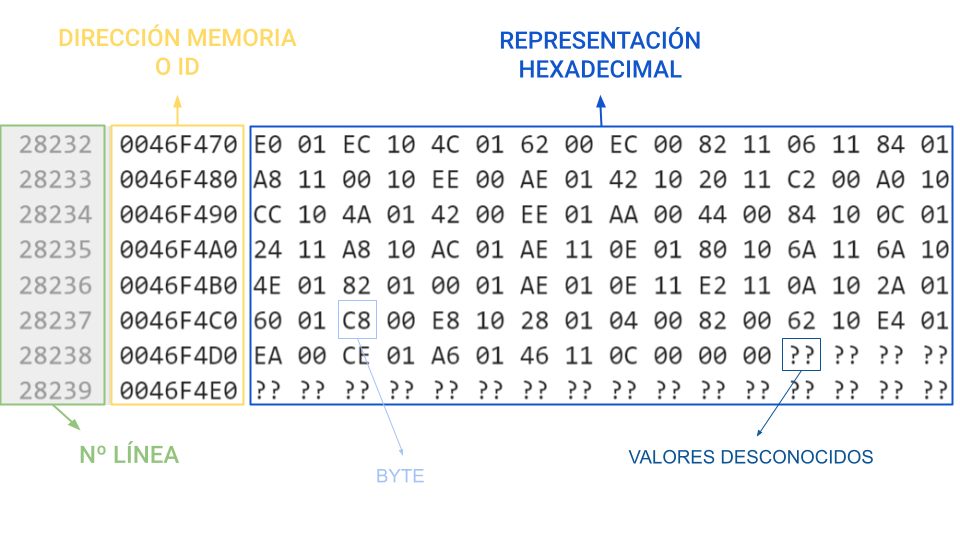
\includegraphics[width=0.7\textwidth]{img/previewMMC.png}
    \end{center}
    \caption{Explicación del contenido de ``0ACDbR5M3ZhBJajygTuf.bytes''.}
    \label{fig:previewMMC}
\end{figure} 


Como aparece en la figura \ref{fig:previewMMC}, los ocho primeros caracteres son direcciones de memoria, seguido de la representación hexadecimal del contenido binario del programa, que contiene 16 bytes (cada uno dos caracteres). A veces nos podemos encontrar con ``??'' en el lugar de un byte. Este símbolo se utiliza en estos archivos para representar que se desconoce su información porque su memoria no se puede leer \citep{cahyani2022influence}. 


\subsection{Distribución del dataset}

Hay un total de 21.741 programas de malware, pero solo 10.868 de ellos tienen etiquetas. Estos programas pertenecen a una de estas 9 familias de malware: Rammit, Lollipop, Kelihos\_ ver3, Vundo, Simda, Tracur, Kelihos\_ ver1, Obfuscator y Gatak. Según \cite{hu2019machine}, podemos definirlas como: 

  

\begin{enumerate}

\item \textbf{Ramnit} es un malware tipo gusano que infecta archivos ejecutables de Windows, archivos de Microsoft Office y archivos HTML. Cuando se infectan, el ordenador pasa a formar parte de una red de \textit{bots} controladas por un nodo central de forma remota. Este malware puede robar información y propagarse a través de conexiones de red y unidades extraíbles.

\end{enumerate}


\begin{wrapfigure}{l}{0.33\textwidth}
  \begin{center}
    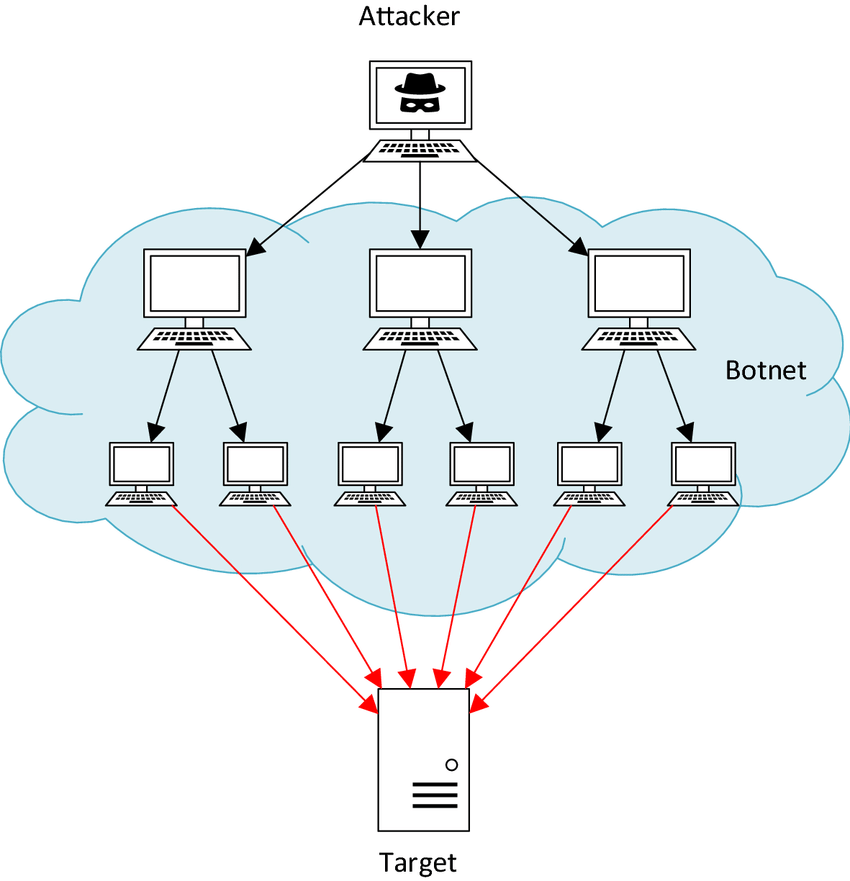
\includegraphics[width=0.33\textwidth]{img/botnetStructure.png}
  \end{center}
    \caption{Estructura de un \textit{botnet}. Imagen sacada de \citep{botnetstructure}.}
  \label{fig:botnetstructure}
\end{wrapfigure}
\vspace{-\baselineskip}

\bigskip
\textbf{2.} \textbf{Lollipop} es un tipo de programa \textit{adware}\footnote{Es una variedad de malware que muestra anuncios no deseados a los usuarios, típicamente como ventanas emergentes o \textit{banners}.} que muestra anuncios no deseados en los navegadores web. También puede redirigir los resultados de búsqueda a recursos web ilegítimos, descargar aplicaciones maliciosas y robar la información del ordenador monitorizando sus actividades web. Este \textit{adware} se puede descargar desde el sitio web del programa o empaquetarse con algunos programas de terceros.


\textbf{3.} \textbf{Simda} es un troyano \textit{backdoor}\footnote{Un \textit{backdoor} permite que una entidad no autorizada tome el control completo del sistema de una víctima sin su consentimiento.} que infecta ordenadores descargando y ejecutando archivos arbitrarios que pueden incluir malware adicional. Los ordenadores infectados pasar a ser parte de una \textit{botnet}, lo que les permite cometer acciones criminales como robo de contraseñas, credenciales bancarias o descargar otros tipos de malware.

\textbf{4.} \textbf{Vundo} es otro troyano conocido por causar publicidad emergente para programas de antivirus falsos. A menudo se distribuye como un archivo DLL(Dynamic Link Library) \footnote{Una parte del programa que se ejecuta cuando una aplicación se lo pide. Se suele guardar en un directorio del sistema.} y se instala en el ordenador como un Objeto Auxiliar del Navegador (BHO) sin su consentimiento. Además, utiliza técnicas

\begin{enumerate}
\item[] avanzadas para evitar su detección y eliminación.
\item[5.] \textbf{Kelihos\_ ver3} es un troyano tipo \textit{backdoor} que distribuye correos electrónicos que pueden contener enlaces falsos a instaladores de malware. Consta de tres tipos de \textit{bots} \citep{kerkers2014characterisation}: controladores (operados por los dueños y donde se crean las instrucciones), enrutadores (redistribuyen las instrucciones a otros \textit{bots}) y trabajadores (ejecutan las instrucciones).

\item[6.] \textbf{Tracur} es un descargador troyano que agrega el proceso 'explorer.exe' a la lista de excepciones del \textit{Firewall} de Windows para disminuir deliberadamente la seguridad del sistema y permitir la comunicación no autorizada a través del \textit{firewall}. Además, esta familia también te puede redirigir a enlaces maliciosos para descargar e instalar otros tipos de malware.

\item[7.] \textbf{Kelihos\_ ver1} es una versión más antigua del troyano Kelihos\_ ver3, pero con las mismas funcionalidades.

\item[8.] \textbf{Obfuscator.ACY} es un tipo de malware sofisticado que oculta su propósito y podría sobrepasar las capas de seguridad del software.  Se puede propagar mediante archivos adjuntos de correo electrónico, anuncios web y descargas de archivos. 
\item[9.] \textbf{Gatak} es un troyano que abre una puerta trasera en el ordenador. Se propaga a través de sitios web falsos que ofrecen claves de licencias de productos. Una vez infectado el sistema, Gatak recopila información del ordenador.
\end{enumerate} 

Como ya mencionamos antes, solo hay 10.868 programas con etiquetas, luego vamos a hacer el análisis descriptivo de los datos solo con estos archivos. De estos programas, solo son válidos 10.860 porque en los 8 archivos restantes\footnote{Los identificadores de estos archivos son 58kxhXouHzFd4g3rmInB, 6tfw0xSL2FNHOCJBdlaA, a9oIzfw03ED4lTBCt52Y, cf4nzsoCmudt1kwleOTI, d0iHC6ANYGon7myPFzBe, da3XhOZzQEbKVtLgMYWv, fRLS3aKkijp4GH0Ds6Pv, IidxQvXrlBkWPZAfcqKT.} (pertenecientes a la familia Ramnit), todo sus bytes son ``??'', es decir, información desconocida. Con estos datos, vamos a ver gráficamente como se distribuyen en las 9 clases de malware (Figura \ref{img: circularMMC}).

\begin{figure}[h]
    \begin{center}
    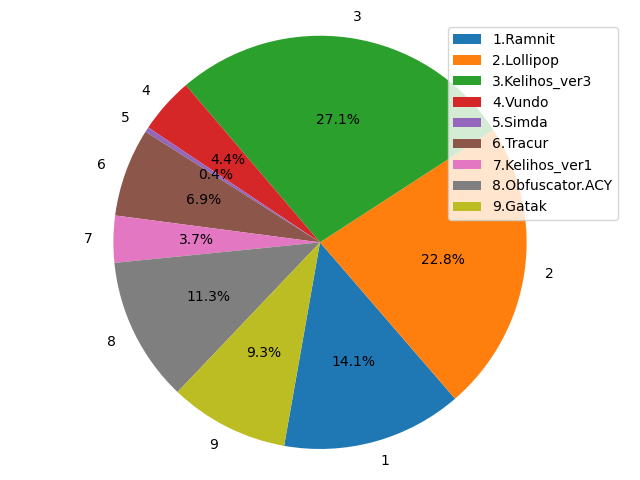
\includegraphics[width=0.6\textwidth]{img/circularMMC.png}
    \end{center}
    \caption{Distribución del BIG 2015 \textit{training} dataset.}
    \label{img: circularMMC}
\end{figure}  

Analizando la Figura \ref{img: circularMMC}, podemos observar como la distribución entre las clases no es uniforme. Mientras que de la clase Simbda hay 42 muestras, de la clase Kelihos\_ ver3 hay 2.942, es decir, 70 veces más de muestras. En \citep{kebede2017classification} deciden prescindir de esta clase, pero nosotros hemos decidido hacer el análisis con las 9 clases. 


A la hora de crear nuestros modelos, hemos dividido el conjunto de datos aleatoriamente usando la función \lstinline|train_test_split()| en grupos del 75\%, 15\% y 10\% para entrenamiento, test y validación respectivamente. La tabla \ref{tab:malware_distribution} muestra como quedarían distribuidas las clases en los diferentes grupos.

\begin{table}[h]
\centering
\begin{tabular}{lccccccccc}
\hline
& Ramnit & Lollipop & Kelihos3 & Vundo & Simda & Tracur & Kelihos1 & Obfus & Gatak \\
\hline
Total & 1533 & 2478 & 2942 & 475 & 42 & 751 & 398 & 1228 & 1013 \\
Train & 1177 & 1835 & 2228 & 337 & 26 & 543 & 306 & 925 & 768 \\
Test & 223 & 394 & 436 & 75 & 9 & 124 & 42 & 177 & 149 \\
Valid & 133 & 249 & 278 & 63 & 7 & 84 & 50 & 126 & 96 \\
\hline
\end{tabular}
\caption{Distribución de los tipos de malware en los conjuntos de datos}
\label{tab:malware_distribution}
\end{table}

 


Para abordar este problema de clasificación, vamos a realizar dos modelos de aprendizaje automático diferentes para luego comparar sus resultados. El primer método que vamos a utilizar es una \acrfull{cnn}. El segundo será entrenar un \textit{autoencoder} junto con una capa de clasificación, primero obteniendo una representación comprimida de los datos y después clasificando esta representación con una red neuronal profunda. 
 







\section{Red Neuronal Convolucional} \label{3.cnn}

Para abordar este problema utilizando como modelo una CNN, solo podemos utilizar los datos etiquetados ya que este método es un método supervisado. Como ya vimos en la sección \ref{sec:2.CNN}, para entrenar estas redes neuronales es necesario tener los datos en forma matricial. Uno de los principales motivos para convertir el malware en imagen es porque los creadores de malware suelen modificar sus implementaciones para producir nuevo malware \citep{nataraj2015sattva}, pero si lo representamos de forma matricial, estos pequeños cambios pueden ser detectados fácilmente \citep{kalash2018malware}.

\subsection{Visualizar el malware como imagen}
Para visualizar los archivos .bytes como imagen en escala de grises, cada byte debe ser interpretado como un píxel en la imagen. Inspirado en \citep{nataraj2011malware}, para pasar de código hexadecimal a imagen primero pasamos cada byte a su número decimal correspondiente que se encuentra en el rango [0,255]\footnote{Cada valor en este intervalo tiene un color asociado donde 0 es el negro y 255 el color blanco.}. Como vimos en el apartado anterior, hay algunos bytes que son ``??'' lo que significa que se desconoce su información. Para solucionar este problema con los datos, en el apéndice B de \citep{geron2022hands}, se plantea eliminar estos caracteres y tratar el resto de bytes. Otra solución la proponen Narayanan et al. \citep{narayanan2016performance}, que es sustituir estos bytes por el valor 255 (color blanco). Después de probar con ambas propuestas y además la de cambiando el ``??'' por el valor 0, finalmente hemos decidido sustituirlo por 0 (color negro) en base a los resultados obtenidos. 

\begin{figure}[h]
    \begin{center}
    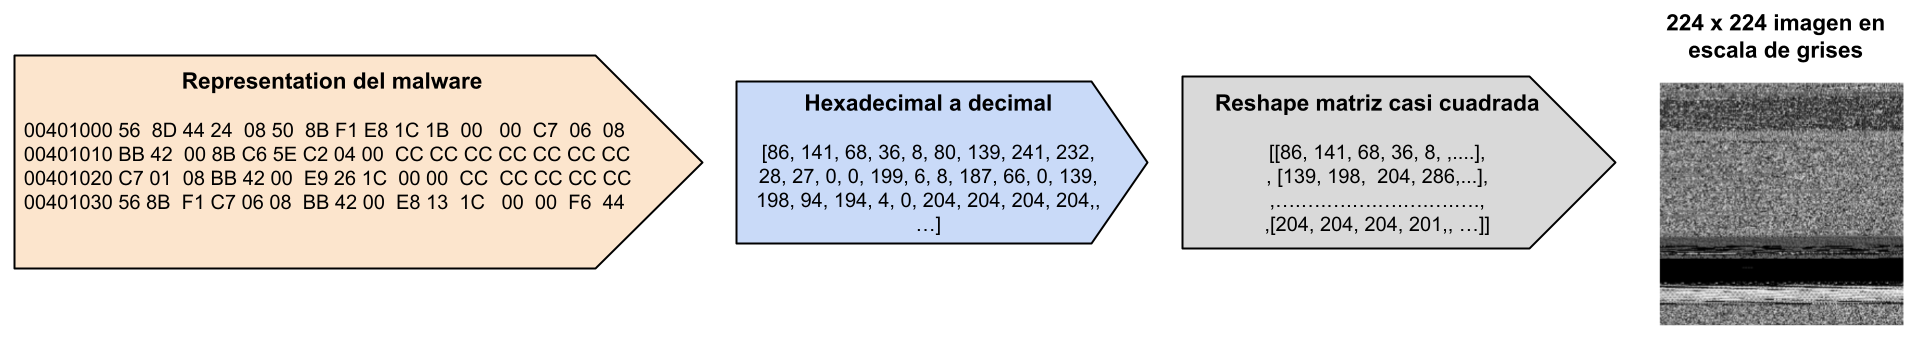
\includegraphics[width=\textwidth]{img/visualMalware.png}
    \end{center}
    \caption{Proceso de visualización del malware. Adaptación de \citep{nataraj2011malware}}
    \label{img: visualMalware}
\end{figure}

Después de tener todos los bytes agrupados en un vector con sus elementos en formato decimal, hacemos un reshape a una matriz 2D de forma que se consiga una matriz lo más cuadrada posible. Como las dimensiones de cada archivo son diferentes, las dimensiones después de hacer el reshape también lo serán, luego tenemos que fijar un tamaño fijo para poder entrenar nuestra CNN \citep{kumar2021mcft}. Para ello, siguiendo el ejemplo de \citep{kalash2018malware}, decidimos escoger como tamaño $224 \times 224$. Para obtener estas dimensiones, Simonyan et al. \citep{simonyan2014very} deciden recortar aleatoriamente un cuadrado de la imagen de tamaño $224 \times 224$, pero nosotros hemos decidido usar interpolación bilineal en base al artículo \citep{he2019malware}. En la figura \ref{img: visualFamilias}, se puede observar cuales son los patrones que sigue cada tipo de malware en su forma matricial.

\begin{figure}[h]
    \begin{center}
    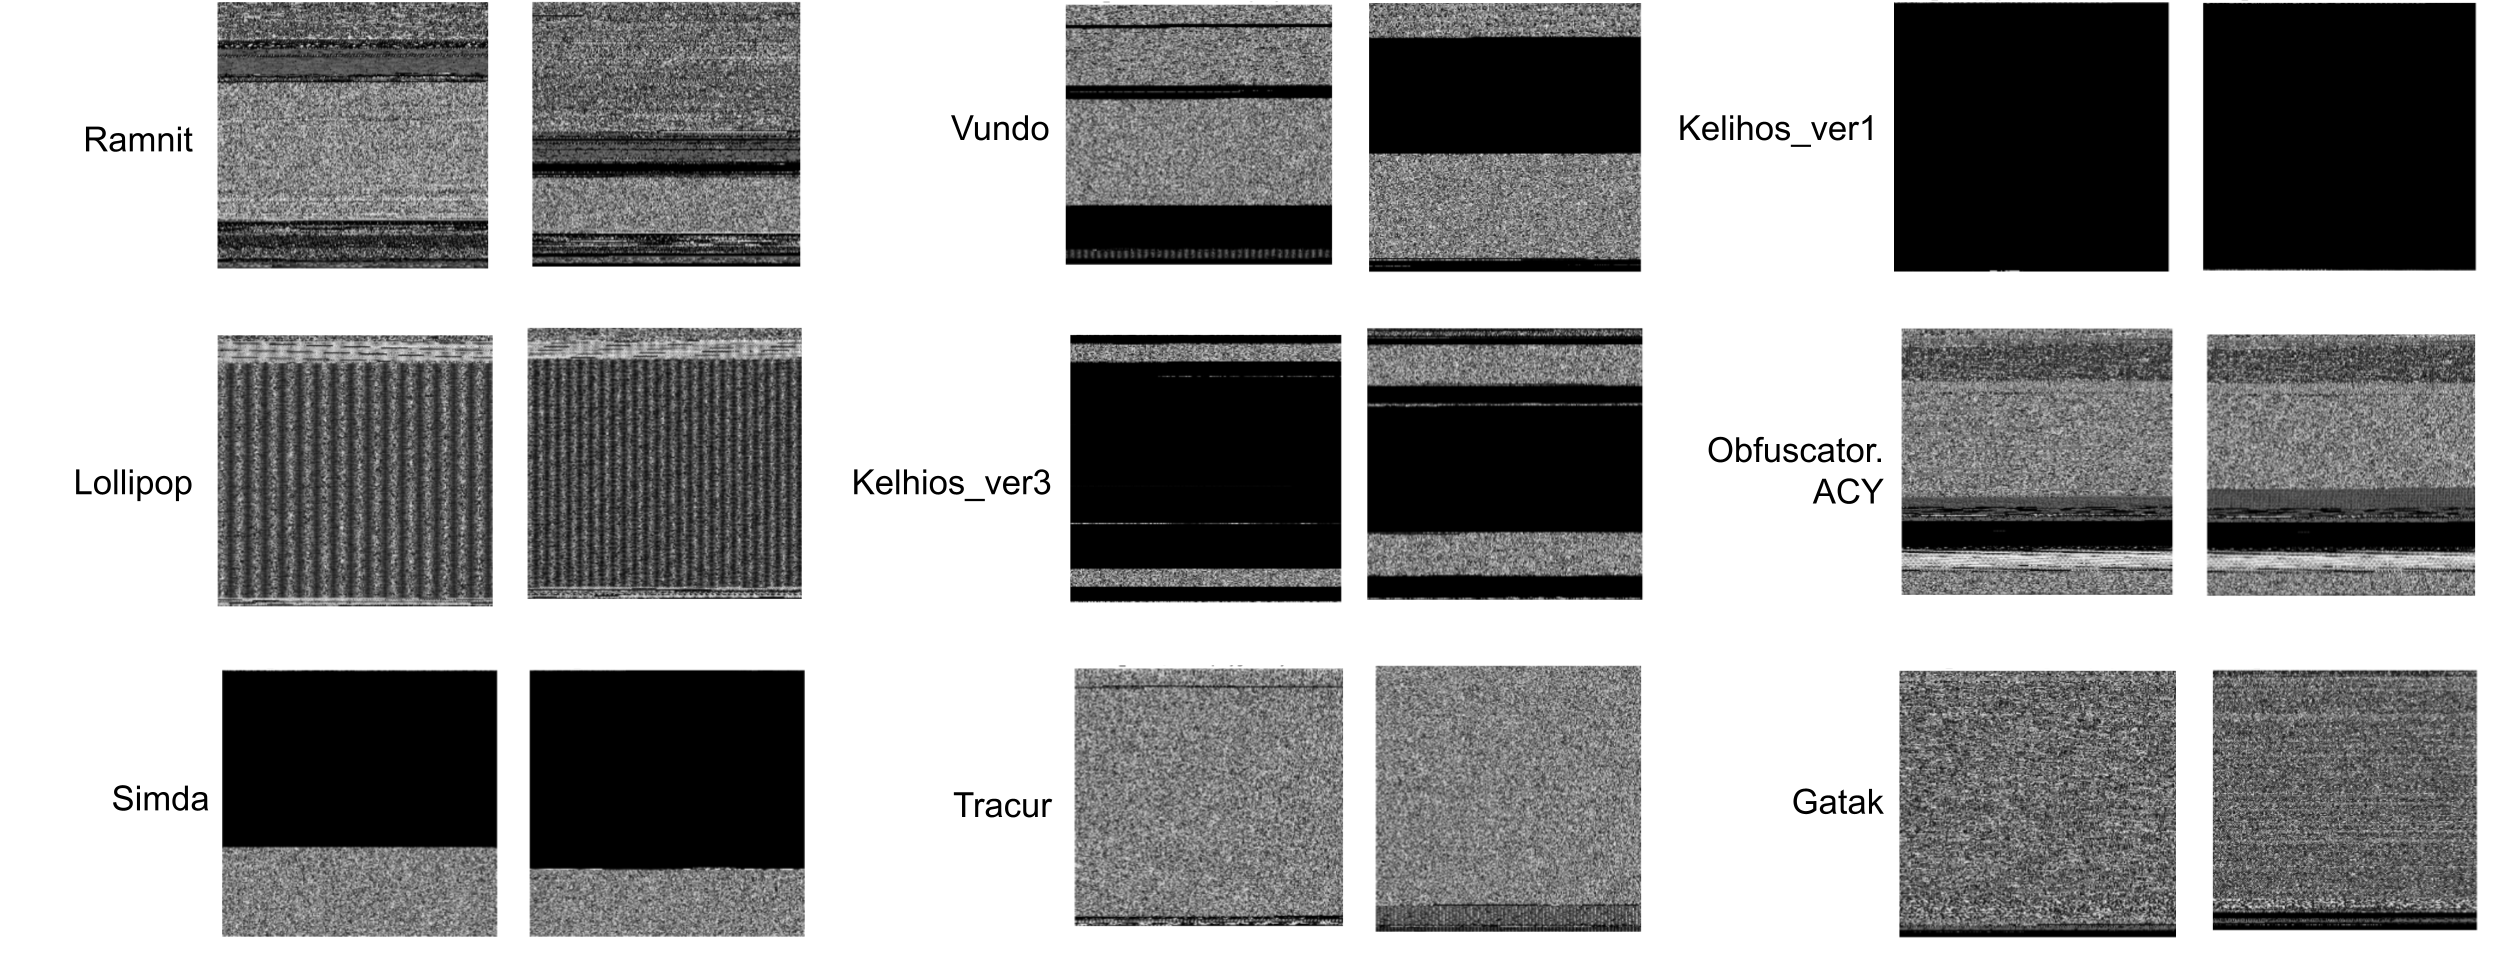
\includegraphics[width=\textwidth]{img/visualFamilias.png}
    \end{center}
    \caption{Visualización familias malware.}
    \label{img: visualFamilias}
\end{figure}


\subsection{Visualización del modelo} \label{sec: visMalware}


Una vez ya hemos explorado y preparado los datos, el siguiente paso es crear nuestra red neuronal convolucional. Para ello hemos seguido el artículo \citep{kalash2018malware}, en el que se crea una M-CNN (malware CNN) con múltiples capas. Vemos su arquitectura en la Figura \ref{img: cnnMMC}.

\begin{figure}[h]
    \begin{center}
    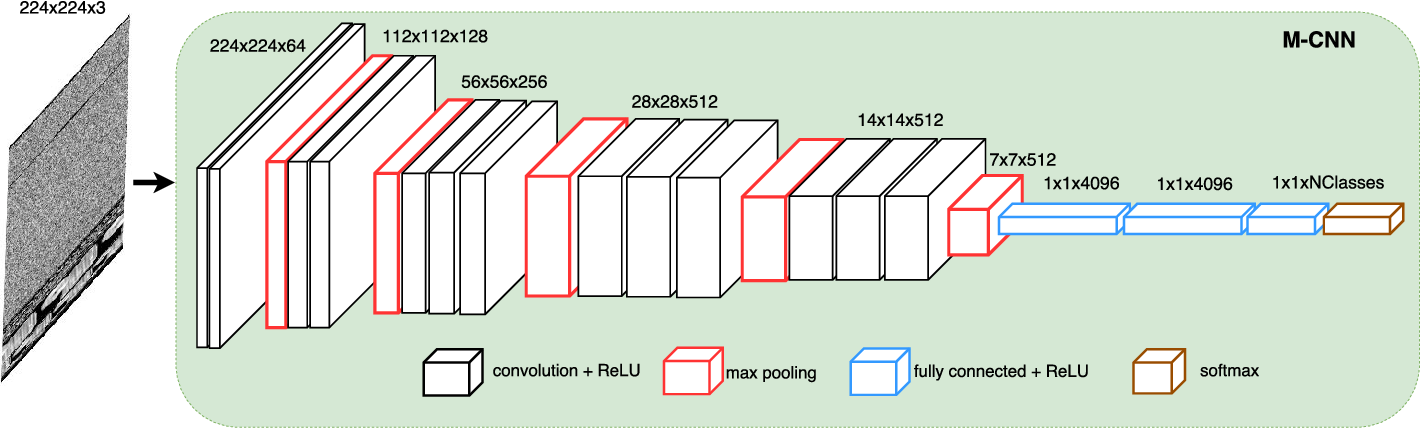
\includegraphics[width=\textwidth]{img/cnnMMC.png}
    \end{center}
    \caption{Arquitectura de la CNN. Fuente \citep{kalash2018malware}.}
    \label{img: cnnMMC}
\end{figure}

En las capas iniciales, se aplican filtros de tamaño $3 \times 3$, que permiten extraer características locales importantes de la imagen de entrada. Las capas convolucionales aprenden a detectar bordes, texturas y otros patrones básicos al principio, y conforme se agregan más capas, las características detectadas se vuelven más abstractas y complejas \citep{geron2022hands}. Después de cada operación de convolución, se aplica la función de activación ReLU para introducir no linealidad en el modelo.

Las capas de \textit{max pooling} reducen la dimensionalidad de los mapas de características seleccionando el valor máximo en subregiones de $2 \times 2$, lo que no solo reduce la carga computacional sino que también ayuda a hacer las características más robustas a pequeñas variaciones y traslaciones en la imagen de entrada \citep{geron2022hands}.

La secuencia de capas convolucionales y de \textit{pooling} se repite varias veces hasta obtener un conjunto final de características que es una matriz de $7 \times 7$ con 512 mapas de características. Esta salida se aplana para convertirla en un vector unidimensional, que luego pasa a través de varias capas completamente conectadas (\textit{fully connected layers}). Finalmente, la capa de salida utiliza una función de activación softmax para generar las predicciones finales del modelo.

Una vez definida la arquitectura de la red, procedemos a compilar y entrenar el modelo. Para la compilación del modelo, hemos seguido el artículo \citep{kalash2018malware} para la elección de las funciones de pérdida y de optimización, con los parámetros adecuados. Utilizamos el optimizador SGD con un \textit{learning rate} inicial de 0.001. Este valor se reduce en un factor de 10 cada 20 \textit{epochs}. Además, fijamos el \textit{momentum} en 0.9 y el \textit{weight decay} en 0.0005. La función de pérdida utilizada es \lstinline|categorical_crossentropy| ya que nuestro problema involucra múltiples clases de etiquetas \citep{categoriCE}.

El entrenamiento se realizó con un \textit{batch size} de 8 y se ejecutó durante 25 \textit{epochs}. Utilizamos \textit{callbacks} para ajustar dinámicamente el \textit{learning rate}, detener el entrenamiento temprano si no se observan mejoras en la pérdida de validación (\lstinline|EarlyStopping|), y registrar los resultados de las métricas utilizadas durante el entrenamiento. Además, se barajea el conjunto de datos de entrenamiento antes de cada \textit{epoch}. 


Después de las 25 \textit{epochs}, este modelo obtiene un \textit{accuracy} en el conjunto de validación del 0.959, mientras que en el conjunto de entrenamiento obtiene 1,0. Por otro lado, en la función de pérdida se obtiene un 0.331 en el conjunto de validación y un 0.0005 en el conjunto de entrenamiento. En la figura \ref{img: dropout0} podemos visualizar la evolución de ambas métricas a lo largo de las 25 iteraciones. En ellas se puede observar como durante las primeras épocas el modelo esta generalizando bastante bien debido a la similitud en los resultados obtenido. Sin embargo a partir de la época 5 se puede observar como tanto el \textit{accuracy} como el \textit{loss} de validación se estabiliza en el 0.94 y 0.3 respectivamente mientras los de entrenamiento siguen optimizándose. Estas diferencias significativas en los resultados de ambos conjuntos de datos, unido al análisis gráfico, nos sugieren que se puede estar produciendo un sobreajuste de los datos de aprendizaje, lo que evita la generalización. 

\begin{figure}[h]
    \begin{center}
    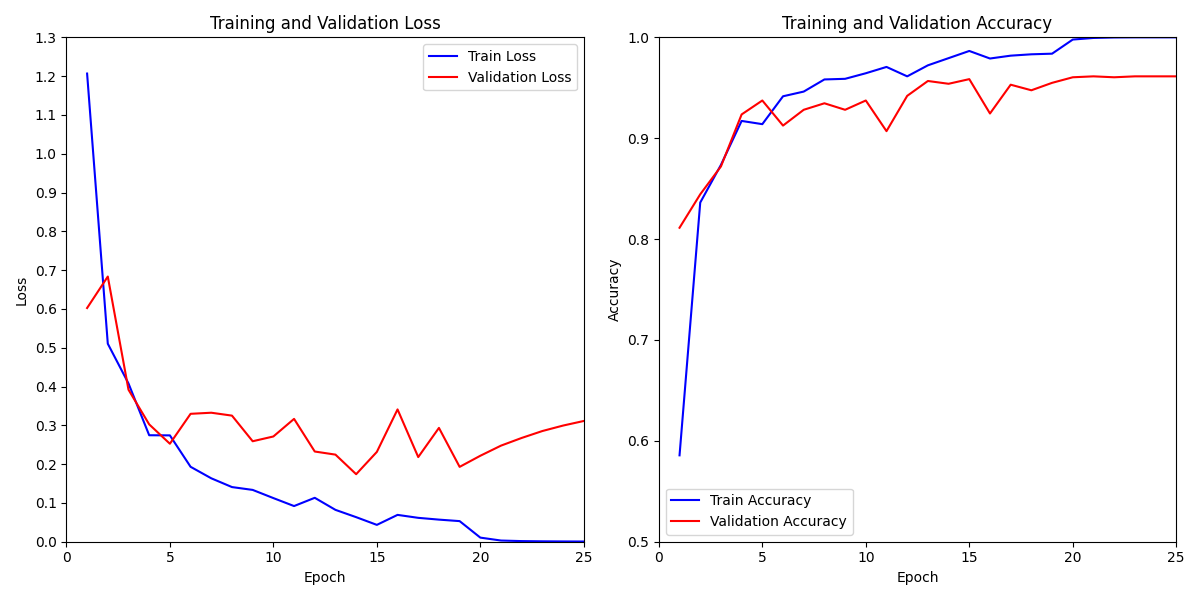
\includegraphics[width=0.6\textwidth]{img/malware_classifier_dropout0.png}
    \end{center}
    \caption{Evolución del modelo en términos de \textit{accuracy} y \textit{loss} siguiendo los pasos del artículo \citep{kalash2018malware}.}
    \label{img: dropout0}
\end{figure}

\subsection{Aportaciones al modelo} \label{subsec:cnnmmc}

Dado los resultados obtenidos previamente, intentaremos mejorar nuestro modelo. Primero de todo, trataremos de aplicar algunas de las técnicas mencionadas en el capítulo \ref{Capitulo_2} para lograr un mejor ajuste de los datos al modelo y obtener una mejor generalización. A continuación, se realizaran diferentes experimentos para comprobar que los hiperparámetros indicados en el artículo \citep{kalash2018malware} son los que mejores resultados obtiene. 


\subsubsection*{Evitar el sobreajuste del modelo}

Primero, vamos a añadir capas de \textit{dropout} después de cada capa densa, como se sugiere en \citep{hinton2012improving, dileep2020dense}. Probaremos con diferentes tasas de \textit{dropout} (0.25, 0.4, 0.5 y 0.6) para determinar cuál proporciona los mejores resultados.

El primer experimento va a consistir en añadir estas capas de \textit{dropout} con una tasa de 0.25. Los resultados obtenidos se muestran en la Figura \ref{fig:cnn25}. Observamos como el modelo generaliza bien hasta la época 7, pero a partir de esa época, empieza a sobreajustar los datos de entrenamiento. Al final de entrenamiento alcanza 1.0 y 0.962 en entrenamiento y validación respectivamente para el  \textit{accuracy}, y un valor en la función de pérdida de 0.0008 y 0.2479 en los datos de entrenamiento y validación respectivamente. Aunque hemos mejorado en términos de generalización y resultados finales después de 25 épocas, incrementaremos la tasa de \textit{dropout} a 0.4 para observar los efectos.

\begin{figure}[h]
    \centering
    \begin{minipage}{0.45\textwidth}
        \centering
        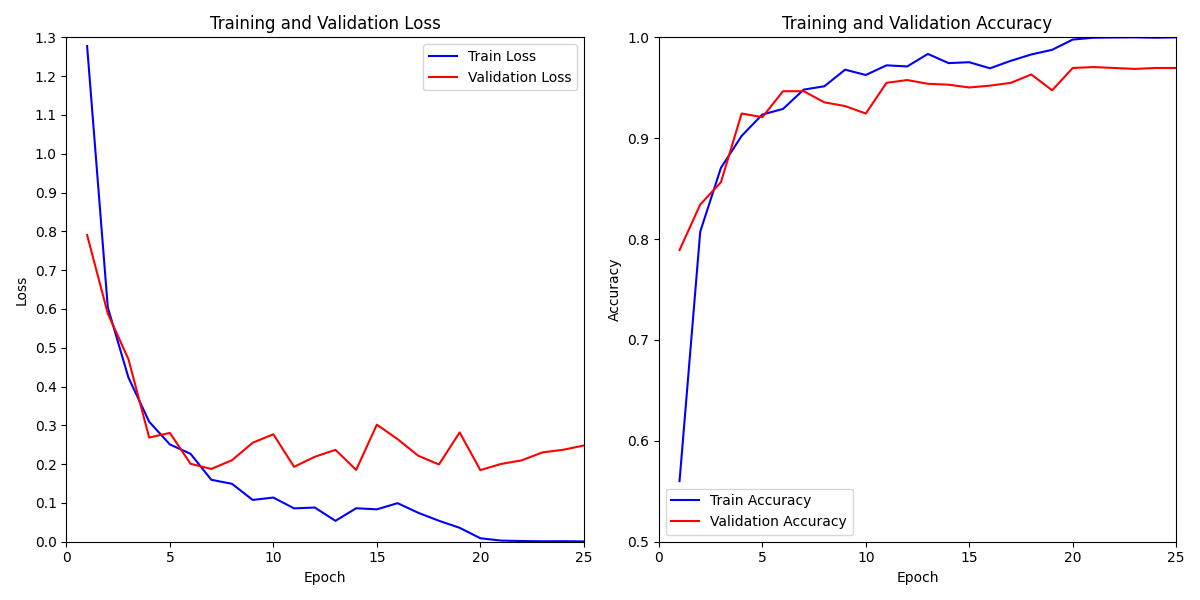
\includegraphics[width=\textwidth]{img/malware_classifier_dropout25.png} % Cambia la ruta por la de tu imagen
        \caption{Evolución del modelo en términos de \textit{accuracy} y \textit{loss} con \textit{dropout} 0.25.}
        \label{fig:cnn25}
    \end{minipage}\hfill
    \begin{minipage}{0.45\textwidth}
        \centering
        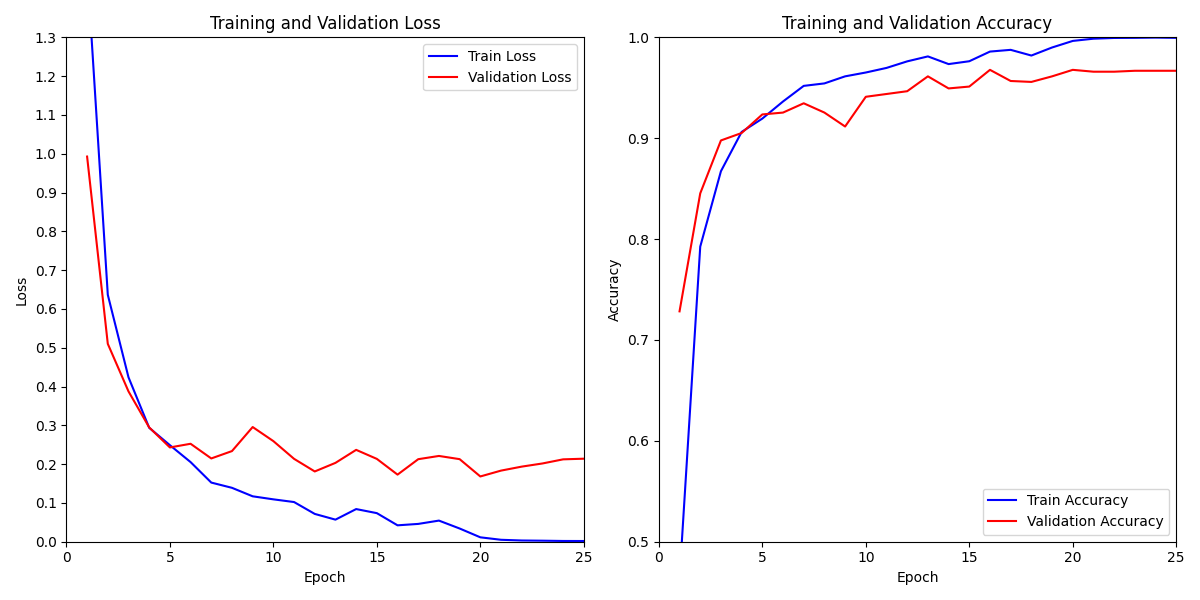
\includegraphics[width=\textwidth]{img/malware_classifier_dropout40.png} 
        \caption{Evolución del modelo en términos de \textit{accuracy} y \textit{loss} con \textit{dropout} 0.4.}
        \label{fig:cnn40}
    \end{minipage}
\end{figure}

Con una tasa de \textit{dropout} de 0.4, como se observa en la Figura \ref{fig:cnn40}, los resultados obtenidos son similares, lo cual nos lleva a probar con una tasa mayor. Al aplicar una tasa de 0.5, observamos en la Figura \ref{fig:cnn50} que el \textit{accuracy} aumenta progresivamente en ambos conjuntos, alcanzando 0.9985 en entrenamiento y 0.9714 en validación. La función de pérdida, por otra parte, muestra una estabilización hasta la época 19 (0.1708), antes de empezar a empeorar, llegando a 0.2614 en la época 25, mientras que la pérdida en entrenamiento sigue descendiendo hasta 0.004.

\begin{figure}[h]
    \centering
    \begin{minipage}{0.45\textwidth}
        \centering
        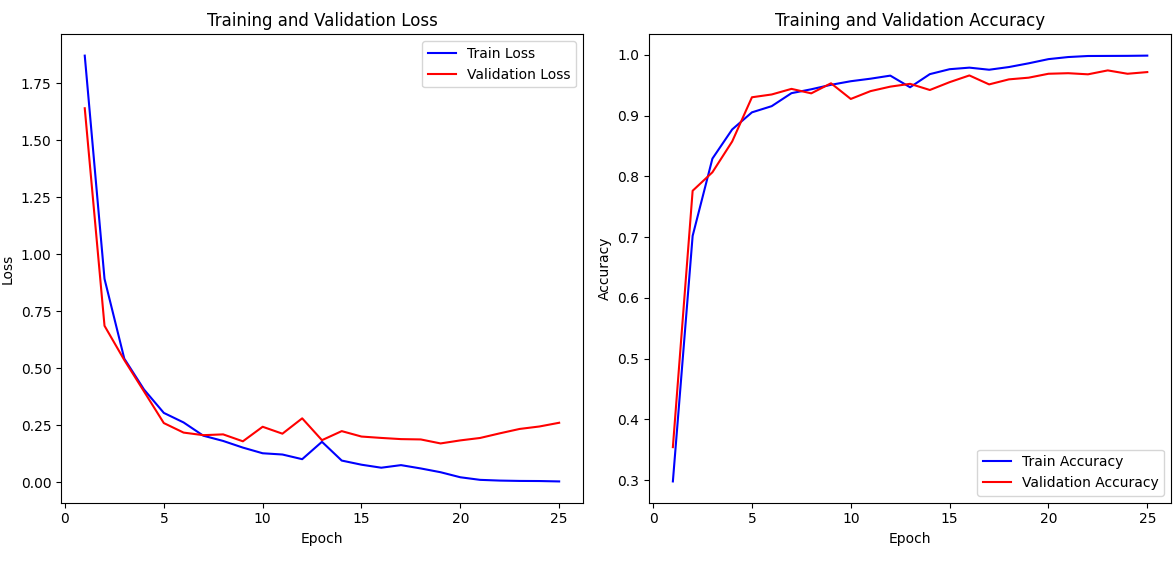
\includegraphics[width=\textwidth]{img/modeloCNN_MMC.png} % Cambia la ruta por la de tu imagen
        \caption{Evolución del modelo en términos de \textit{accuracy} y \textit{loss} con \textit{dropout} 0.5.}
        \label{fig:cnn50}
    \end{minipage}\hfill
    \begin{minipage}{0.45\textwidth}
        \centering
        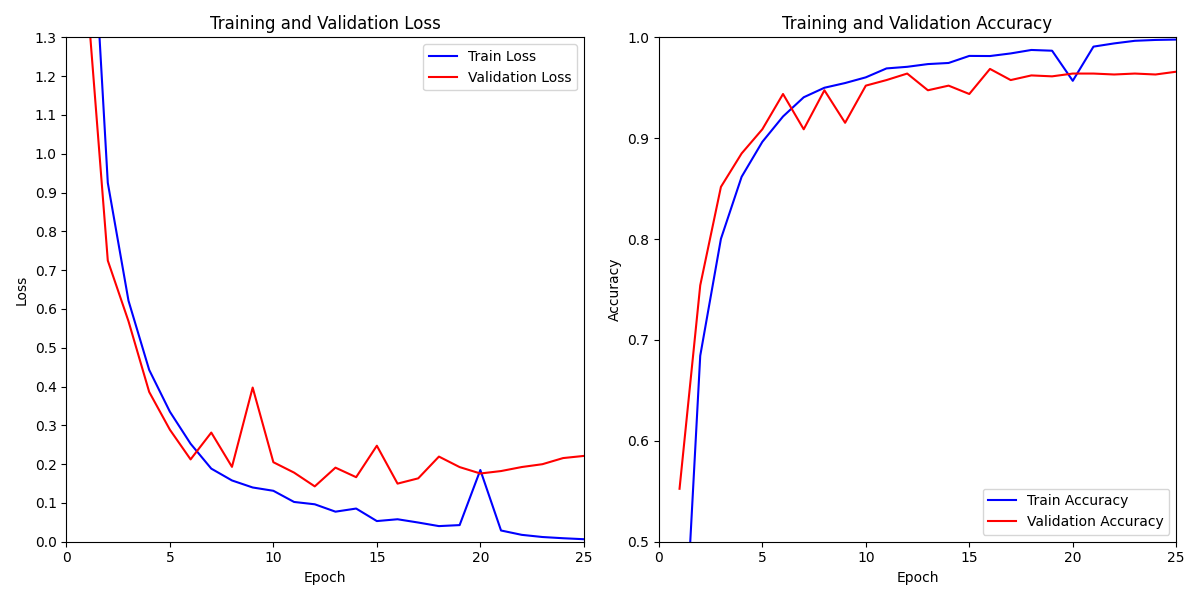
\includegraphics[width=\textwidth]{img/malware_classifier_dropout55.png} 
        \caption{Evolución del modelo en términos de \textit{accuracy} y \textit{loss} con \textit{dropout} 0.55.}
        \label{fig:cnn55}
    \end{minipage}
\end{figure}

Para verificar que esta tasa es la más óptima, probamos con una tasa de 0.55 y, como se muestra en la Figura \ref{fig:cnn55}, obtenemos resultados casi idénticos al caso con una tasa de 0.4. Concluimos que los mejores resultados se obtienen con una tasa de \textit{dropout} del 0.5.

Para evitar el sobreaprendizaje de los datos de entrenamiento, añadimos el \textit{callback} \textit{\lstinline|EarlyStopping|}. Aplicamos esta función a la métrica por defecto \lstinline|val_loss|, con una \lstinline|patience| de 4 épocas. Nuestro entrenamiento se detiene en la época 20 después de alcanzar su mejor valor de pérdida en el conjunto de validación con una pérdida de 0.1716 y un \textit{accuracy} de 0.965, comparado con una pérdida de 0.026 y un \textit{accuracy} de 0.991 en el entrenamiento respectivamente. Aunque este modelo no alcanza el mejor \textit{accuracy}, es el que mejor generaliza los datos. Véase la Figura \ref{fig:cnn50ES}.

\begin{figure}[H]
    \centering
    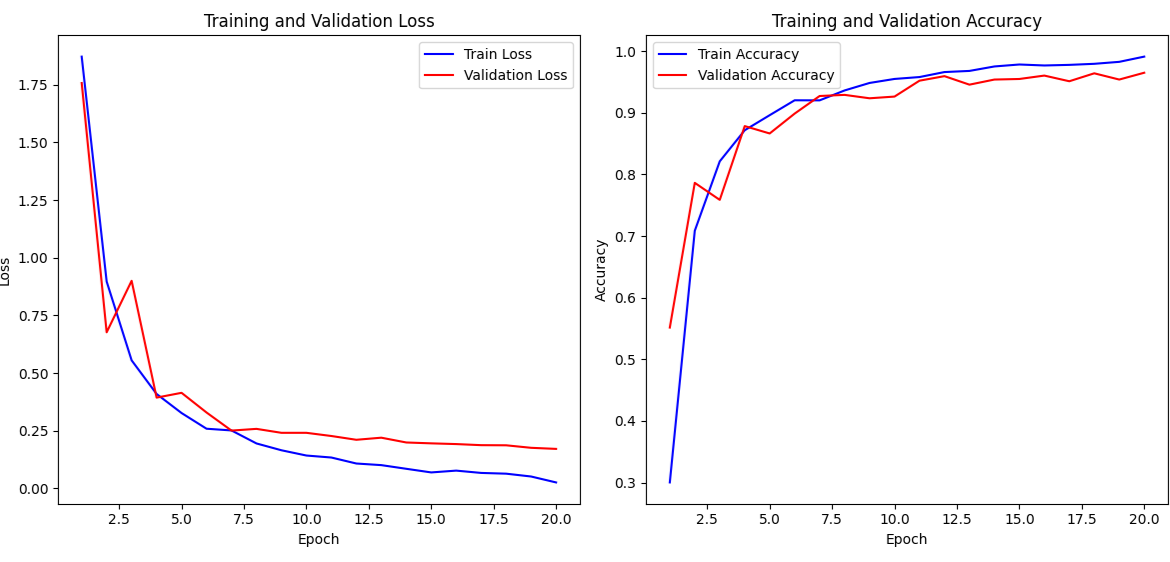
\includegraphics[width=0.6\textwidth]{img/modelo20MMC_CNN.png} 
    \caption{Evolución del modelo en términos de \textit{accuracy} y \textit{loss} con \textit{dropout} 0.5 y \lstinline|EarlyStopping|.}
    \label{fig:cnn50ES}
\end{figure}

Una vez se ha obtenenido el mejor modelo, se van a realizar más experimentos para verificar que efectivamente el resto de hiperparámetros que se han propuesto en el artículo \citep{kalash2018malware} son los que mejor resultados obtiene. Para ello,  se ha probado con un diferente \lstinline|step_decay| (reducir el \textit{learning rate} en 10 unidades cada 10 épocas, 20 épocas o nunca) y con diferentes\textit{ batch sizes} (8, 16 y 32). Para todos estos experimentos, se utilizó la arquitectura explicada anteriormente con una tasa de \textit{dropout} del 0.5 y sin \lstinline|EarlyStopping|.

\subsubsection{Experimentos con diferentes \textit{step decay}}

En esta sección, se analizan tres experimentos realizados con diferentes configuraciones de \textit{step decay} en el entrenamiento de la CNN. Los experimentos variaron en la frecuencia de reducción del \textit{learning rate}: cada 20 épocas, cada 10 épocas, y sin reducción. A continuación, se presentan los resultados obtenidos.


En el \textbf{primer experimento}, se aplicó una reducción del \textit{learning rate} \textbf{cada 20 épocas}, como se menciona en \citep{kalash2018malware}. Los resultados ya han sido estudiados anteriormente ya que son los mismos hiperparámetros que se aconsejaban usar. La reducción del \textit{learning rate} cada 20 épocas permite al modelo ajustar su aprendizaje de forma gradual. En las primeras 20 épocas, el modelo se beneficia de un \textit{learning rate} más alto que permite realizar ajustes significativos a los pesos. Después de la reducción, el \textit{learning rate} más bajo ayuda a afinar estos ajustes, lo que puede mejorar la convergencia y la estabilidad del modelo al evitar grandes oscilaciones en la pérdida. Este enfoque balancea bien la exploración y la explotación durante el entrenamiento.


El \textbf{segundo experimento} redujo el \textit{learning rate} \textbf{cada 10 épocas} (ver Figura \ref{fig:step_decay_10_epochs}). La pérdida en el entrenamiento disminuyó de 1.809 a 0.014 y la precisión aumentó de 33.0\% a 99.6\%. En el conjunto de validación, la pérdida disminuyó de 1.121 a 0.200 y la precisión mejoró de 61.9\% a 96.7\%. Como se observa en la Figura \ref{fig:step_decay_10_epochs}, hasta la época 10 tanto la pérdida como la precisión del conjunto de validación presentan resultados similares al conjunto de entrenamiento, pero a partir de esta época, se estabilizan y dejan de mejorar significativamente.


La reducción del \textit{learning rate} cada 10 épocas puede ser demasiado frecuente, lo que podría limitar la capacidad del modelo para realizar grandes ajustes necesarios al principio del entrenamiento. Esto puede conducir a una estabilización temprana, limitando la mejora de la precisión después de una cierta cantidad de épocas. La reducción más frecuente también puede hacer que el modelo se "acomode" demasiado pronto, antes de haber explorado completamente el espacio de pesos, lo que podría explicar la estabilización observada a partir de la época 10.

\begin{figure}[h]
    \centering
    \begin{minipage}{0.45\textwidth}
        \centering
        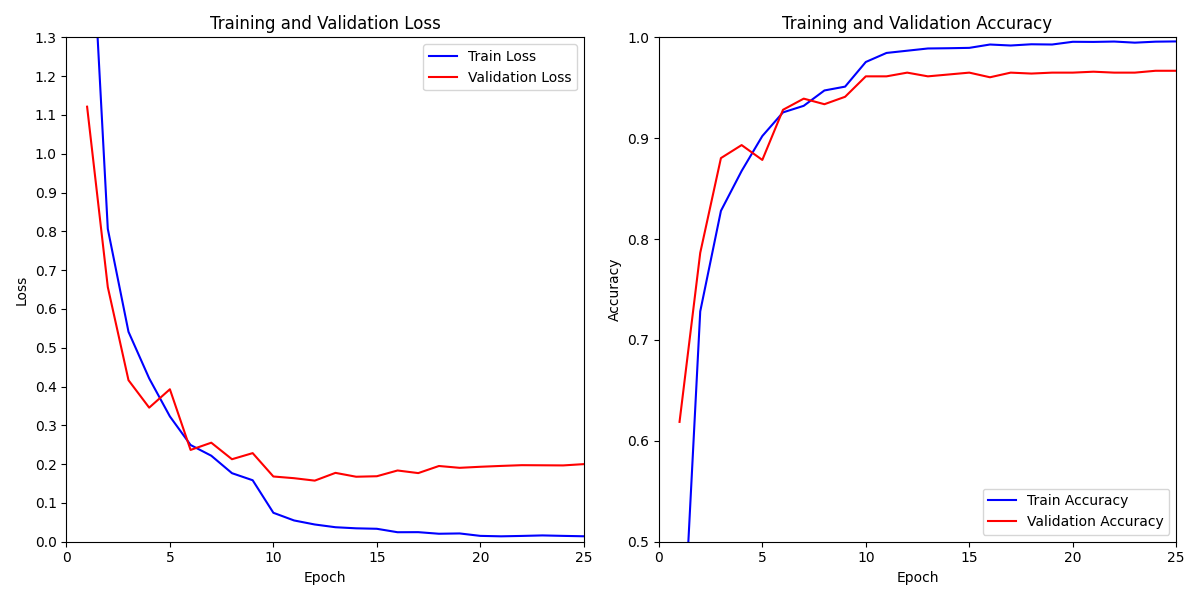
\includegraphics[width=\textwidth]{img/malware_classifier_lr10.png}
        \caption{Resultados para \textit{step decay} cada 10 épocas.}
        \label{fig:step_decay_10_epochs}
    \end{minipage}\hfill
    \begin{minipage}{0.45\textwidth}
        \centering
        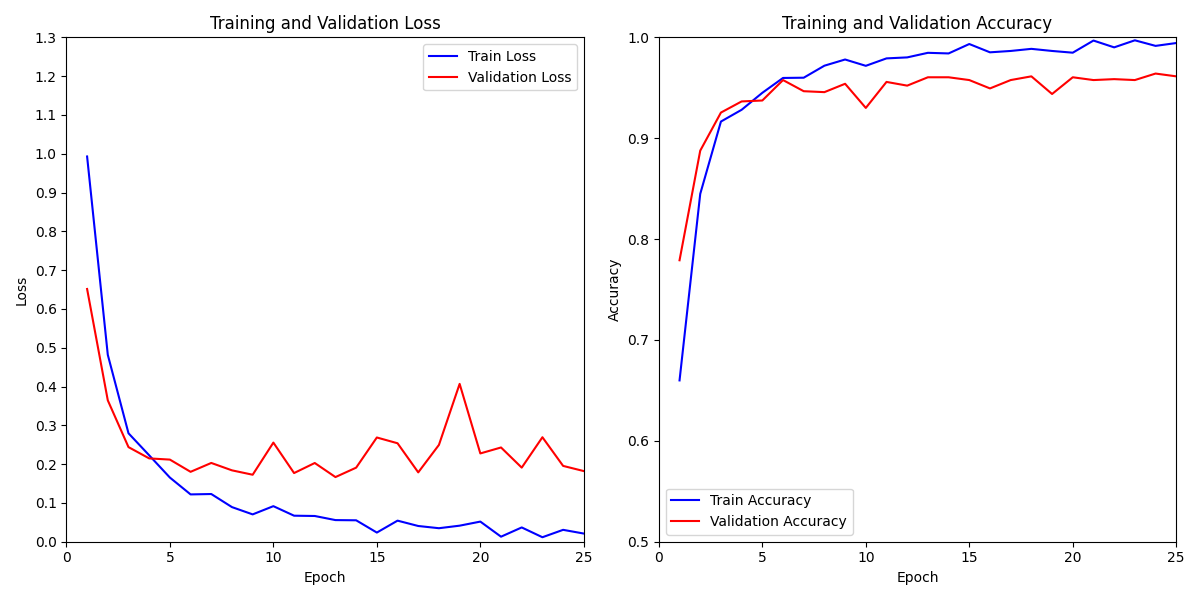
\includegraphics[width=\textwidth]{img/malware_classifier_lr30_droupout0.png}
        \caption{Resultados sin reducción de \textit{step decay}.}
        \label{fig:step_decay_never}
    \end{minipage}
\end{figure}

Finalmente, se realizó un \textbf{experimento sin reducción del \textit{learning rate}} (ver Figura \ref{fig:step_decay_never}). Los resultados fueron inferiores en comparación con los experimentos anteriores. La pérdida en el entrenamiento disminuyó de 1.916 a 0.059 y la precisión aumentó de 26.7\% a 98.3\%. En el conjunto de validación, la pérdida se redujo de 1.918 a 0.184 y la precisión mejoró de 43.6\% a 95.9\%.  Aunque los resultados no son malos, fueron peores en comparación con los otros modelos que aplicaron \textit{step decay}.


No reducir el \textit{learning rate} en ningún momento puede llevar a que el modelo realice ajustes demasiado grandes durante todo el entrenamiento, lo que puede resultar en una convergencia menos precisa. El \textit{learning rate} constante puede ser demasiado agresivo en las últimas etapas del entrenamiento, evitando que el modelo afine los pesos y, por lo tanto, logre una precisión óptima. Esto explica por qué los resultados fueron inferiores, ya que el modelo no se beneficia del refinamiento progresivo que proporciona la reducción del \textit{learning rate}.

En conclusión, el experimento con \textit{step decay} cada 20 épocas obtuvo los mejores resultados en términos de \textit{accuracy} y \textit{loss}, además de mostrar una mejor generalización en los datos de validación.

\subsubsection{Experimentos con diferentes\textit{ batch sizes}} 

Para evaluar el impacto de diferentes \textit{batch sizes}, se realizaron experimentos con \textit{batch sizes} de 8, 16 y 32. Primero, se realizó un experimento con \lstinline|batch_size = 8|, cuyos resultados ya se han discutido en el apartado anterior y en el capítulo \ref{Capitulo_3}. A continuación, se presentan los resultados obtenidos con \lstinline|batch_size = 16| y \lstinline|batch_size = 32|. Los datos de cada experimento se recogen en las Figuras \ref{fig:MMCbatch16} y \ref{fig:MMCbatch32} respectivamente. 

\begin{figure}[h]  
    \centering
    \begin{minipage}{0.45\textwidth}
        \centering
        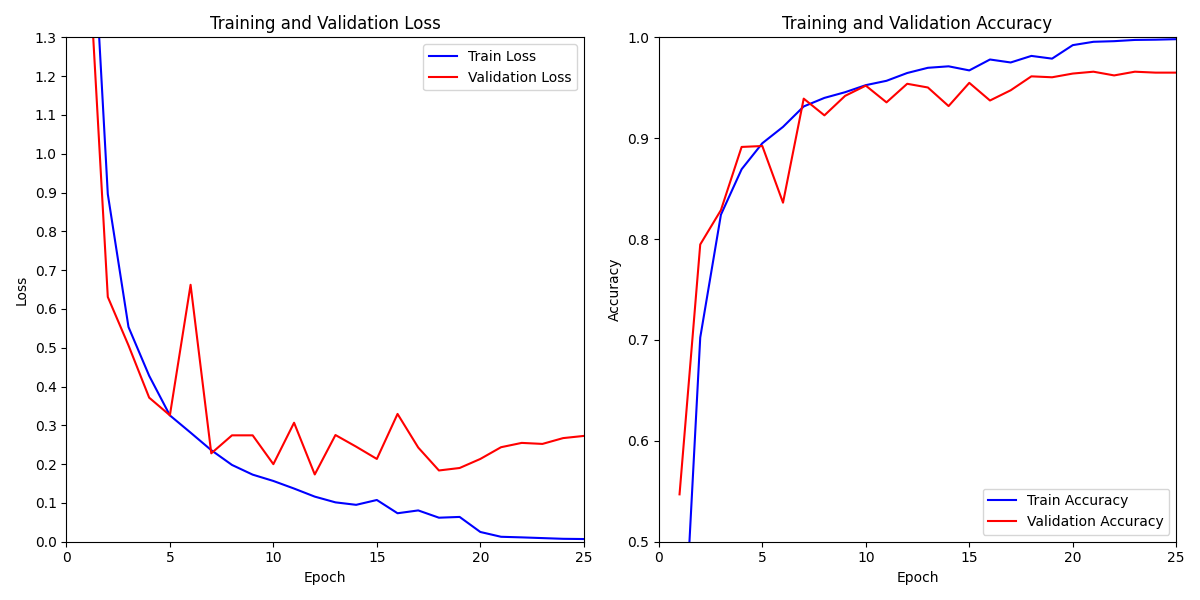
\includegraphics[width=1.1\textwidth]{img/malware_classifier_batch16.png}
        \caption{Entrenamiento y validación del modelo de clasificación usando un \lstinline|batch_size = 16|.}
        \label{fig:MMCbatch16}
    \end{minipage}\hfill
    \begin{minipage}{0.45\textwidth}
        \centering
        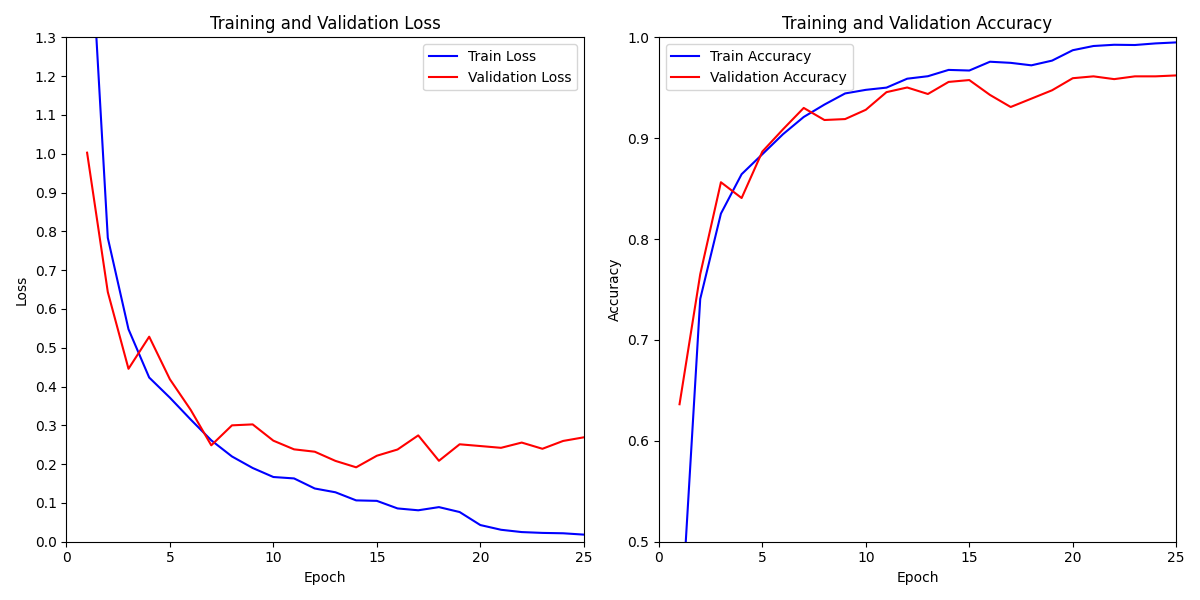
\includegraphics[width=1.1\textwidth]{img/malware_classifier_batch32.png}
        \caption{Entrenamiento y validación del modelo de clasificación usando un \lstinline|batch_size = 32|.}
        \label{fig:MMCbatch32}
    \end{minipage}
\end{figure}

El aumento del \textit{batch size} a 16 mejoró ligeramente la estabilidad del entrenamiento. La pérdida de entrenamiento comenzó en 1.809 y disminuyó a 0.014, mientras que la precisión aumentó de 33.0\% a 99.6\%. En validación, la pérdida se redujo de 1.121 a 0.200, y la precisión mejoró de 61.9\% a 96.7\%. 

Con un \textit{batch size} de 32, la pérdida de entrenamiento comenzó en 1.809 y disminuyó a 0.014, mientras que la precisión aumentó de 33.0\% a 99.6\%. En validación, la pérdida se redujo de 1.121 a 0.200, y la precisión mejoró de 61.9\% a 96.7\%.

Observando las gráficas (Figura \ref{fig:MMCbatch16} y Figura \ref{fig:MMCbatch32}), se puede apreciar que, en términos generales, no hay diferencias significativas entre los \textit{batch sizes} de 16 y 32 en términos medios, si en valores particulares ya que con 16 se pueden observar más fluctuaciones. Sin embargo, comparándolas con la Figura \ref{fig:cnn50} con \lstinline|batch_size = 8|, se observa que este valor ajusta mejor el modelo. Mientras que con \textit{batch sizes} superiores a 8, el modelo deja de aprender características principales a partir de la época 7, con \lstinline|batch_size = 8| esta época se extiende hasta la 12. Los \textit{batch sizes} más grandes pueden llevar a que el modelo se ajuste a los patrones de los lotes en lugar de generalizar adecuadamente a todo el conjunto de datos, lo que podría explicar por qué el modelo deja de aprender características principales después de la época 7, ya que los grandes lotes suavizan demasiado las actualizaciones de los pesos.

En base a estos resultados, verificamos que con un \lstinline|batch_size = 8|, se obtiene los mejores resultados, al igual que con un \textit{step decay} de 10 unidades cada 20 \textit{epochs}, como se había indicado en el artículo \citep{kalash2018malware}.


\section{Autoencoder} \label{sec: 3.AE}

Veamos ahora otro planteamiento para resolver este problema de clasificación de malware. Hemos visto en la sección \ref{sec:ae} que los \textit{autoencoders} son métodos de \textit{machine learning} no supervisados y que entre sus funcionalidades no se encuentra la clasificación. Sin embargo, sus principales utilidades son la reducción de dimensionalidad, la detección de intrusiones o la eliminación de ruido. La motivación detrás del uso de un \textit{autoencoder} es su capacidad para aprender una representación comprimida de los datos de entrada, que luego se puede utilizar para mejorar el rendimiento de un modelo de clasificación usando una secuencia de capas densas \textit{fully connected}. A diferencia del modelo de CNN, no hemos usado de base ningún artículo que ya haya realizado experimentos con un \textit{autoencoder} para resolver este problema de clasificación de malware, sino que todo ha sido trabajo propio. 


Para este método de \textit{machine learning}, vamos a usar todos los datos de la base de datos Microsoft Malware Classification (BIG 2015), tanto los 10.873 programas sin etiquetar como los 10.868 programas de entrenamiento con etiquetas. Primero, se preparan los datos para utilizarlos en el modelo. Para ello, vamos a utilizar el mismo procedimiento explicado en la sección \ref{sec: visMalware} y crearemos imágenes $224 \times 224$ en escala de grises. A continuación, dependiendo de si las entradas del \textit{autoencoder} tiene que ser en imagen o en vector, se aplanarán los datos o no. En segundo lugar, se entrenará el \textit{autoencoder}. La dimensión del cuello de botella es de $4.096$ para que coincida con la dimensión de la primera capa densa de la CNN. Para entrenarla, vamos a utilizar los 21.741 programas disponibles ya que no necesita las etiquetas para entrenarlo, además, el \textit{autoencoder} se entrena minimizando el error cuadrático medio (MSE) entre los datos de entrada y su reconstrucción \citep{guo2017deep}, optimizado con el algoritmo Adam \citep{aekeras}. Una vez se ha entrenado el AE y ya tenemos los parámetros entrenados para obtener una versión comprimida de los datos de entrada, ahora se entrena la segunda parte del modelo, una ANN. Para ello, las primeras capas del ANN se corresponden con el \textit{encoder} entrenado antes. Durante el entrenamiento del clasificador no seguirán entrenándose los pesos y bias de esta primera parte, sino que estos parámetros se bloquean \citep{lopes2022effective}. A continuación de estas capas, se añaden varias capas densas intercaladas con capas de \lstinline|Dropout(0,5)|. Esta parte final coincide con la parte final de la CNN. Para entrenar esta segunda parte del modelo solo se utilizan los 10.860 programas etiquetados.

\begin{figure}[h]
    \begin{center}
    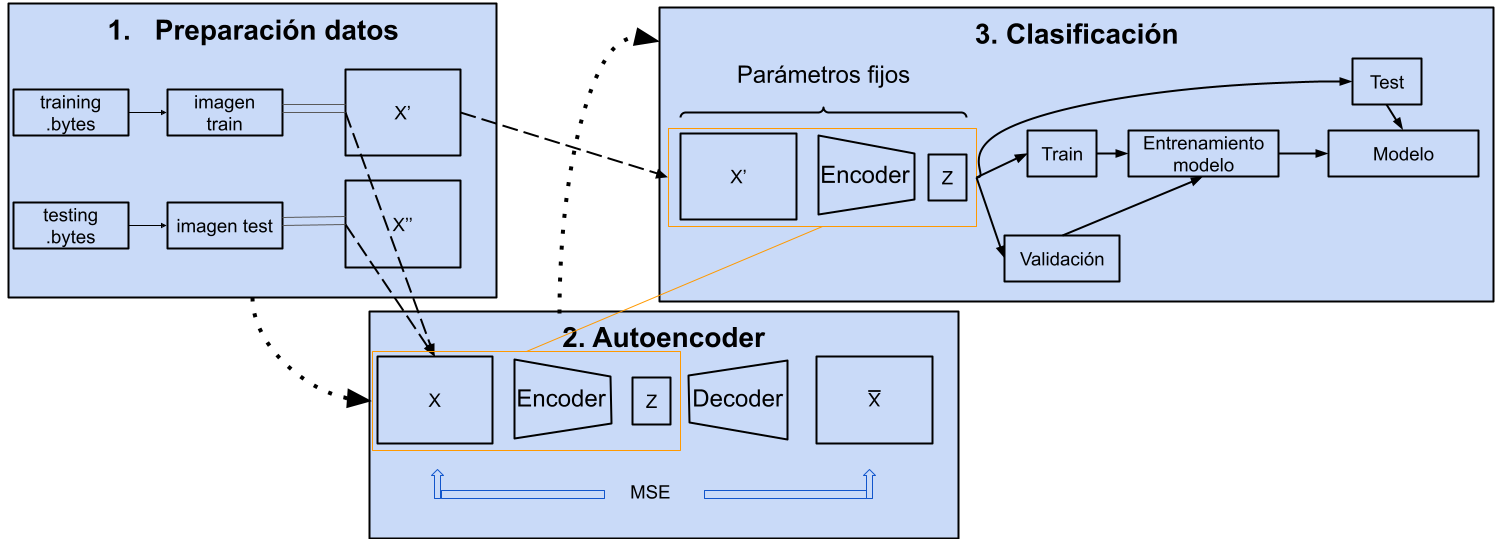
\includegraphics[width=0.9\textwidth]{img/aeMMCgen.png}
    \end{center}
    \caption{Esquema de la arquitectura de un modelo usando como primer paso un \textit{autoencoder}.}
    \label{img: aeMMCgen}
\end{figure}

Para realizar este modelo, se utilizan 3 formas diferentes para comprimir los datos: un \textit{autoencoder} simple, un \textit{autoencoder} con varias capas ocultas y un \textit{autoencoder} convolucional, siguiendo el ejemplo de \citep{aekeras} para reconocimiento de dígitos MNIST. 

\bigskip
\bigskip

\begin{minipage}{0.55\textwidth}
    \subsection{Autoencoder simple}
    
    Para ello, como las capas utilizadas en esta arquitectura son densas, es necesario que los datos de entrada estén aplanados en un vector, luego lo primero que hacemos es preparar los datos para que tengan de dimensión $50.176$. Esta capa se conecta completamente con el cuello de botella $4.096$ que a su vez se vuelve a conectar con otra capa densa de $50.176$ neuronas. Se entrenará este modelo durante 36 épocas y con mini-lotes de 8. Al acabar su entrenamiento, obtenemos una pérdida en los datos de entrenamiento del 0.04598 y en los datos de validación ($20\%$ del total), un 0.04741. 

\end{minipage}
\begin{minipage}{0.02\textwidth}
    \textbf{ }
\end{minipage}
\begin{minipage}{0.35\textwidth}
    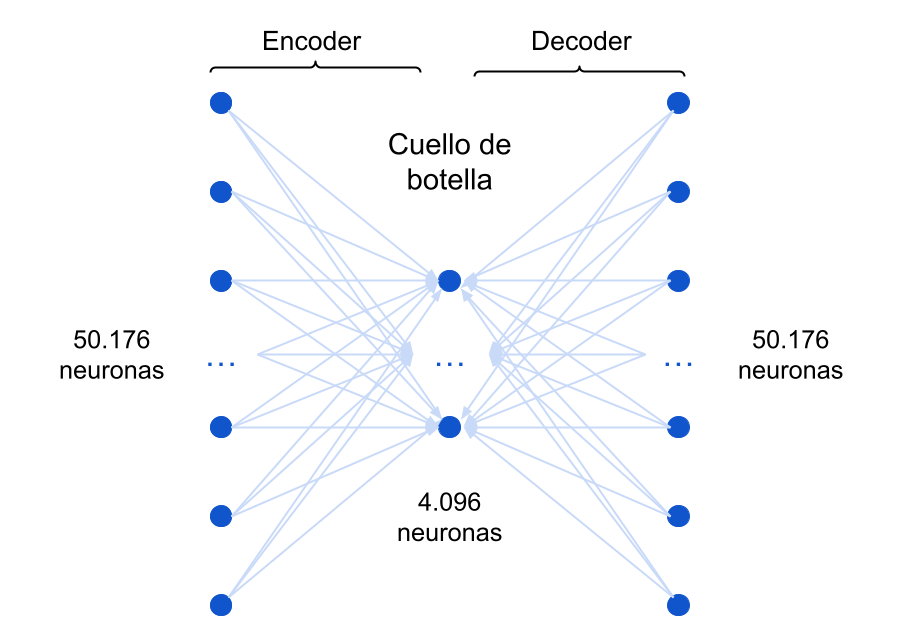
\includegraphics[width=1.1\textwidth]{img/aeMMC.png}
    \captionof{figure}{Esquema de la arquitectura usando un \textit{autoencoder} simple.}
    \label{img: aeMMC}
\end{minipage}

A continuación, se extrae el \textit{encoder} y se agrega una secuencia de 2 capas densas con activación ReLU junto con una capa de \textit{dropout} cada una para evitar el sobreajuste. Para finalizar, se añade una capa densa con 9 neuronas y activación softmax para clasificar  cada una de las instancias. La tasa de \textit{dropout} utilizada es 0,4. Entrenamos el modelo durante 25 épocas con mini-lotes de 8. Además añadimos el \textit{callback} \lstinline|EarlyStopping| con \lstinline|patience = 4| y restaurando los pesos del mejor modelo en caso de parada temprana para prevenir el sobreajuste. El optimizador utilizado para entrenar el modelo de clasificación es el optimizador SGD (\textit{Stochastic Gradient Descent}) con un \textit{learning rate} inicial de 0.001. Además, fijamos el \textit{momentum} en 0.9 y el \textit{weight decay} en 0.0005. En cuanto a la función de pérdida, vamos a hacer 2 experimentos con \lstinline|categorical_crossentropy| y con \lstinline|mse| para comparar el rendimiento de diferentes configuraciones del modelo de clasificación. A continuación, se presentan los resultados de ambos modelos y se determina cuál es el más adecuado.
    
El primer método para comprimir la información de entrada es usando un \textit{autoencoder} simple con una capa oculta que se corresponde con el cuello de botella. La arquitectura de este método se puede observar en la figura \ref{img: aeMMC}

En el primer modelo, se utiliza como función de coste \lstinline|mse|. Podemos observar en la figura \ref{fig:ae_sgd_mse} como muestra una pérdida de entrenamiento y validación que disminuyen consistentemente a lo largo de las épocas, con valores que oscilan entre 0.076 y 0.066. La precisión tanto en entrenamiento como en validación se mantiene alrededor de 0.6, lo que indica una capacidad limitada del modelo para generalizar. Aunque el modelo es estable y no muestra signos de sobreajuste, la precisión relativamente baja sugiere que podría beneficiarse de una arquitectura más compleja o de más datos de entrenamiento.

\begin{figure}[h]
    \centering
    \begin{minipage}{0.45\textwidth}
        \centering
        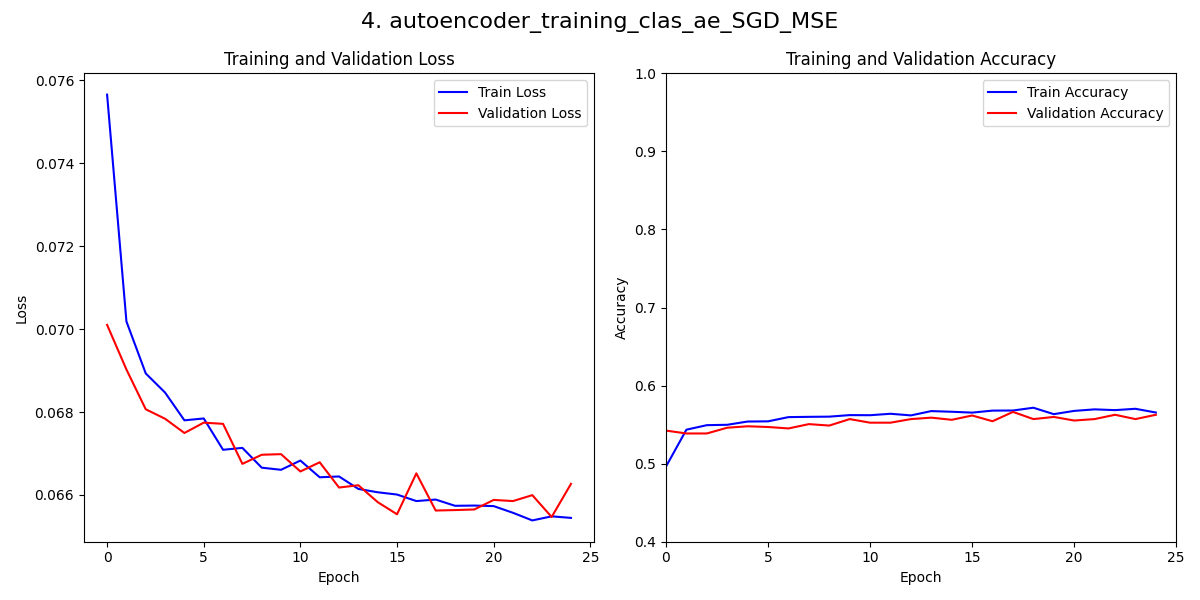
\includegraphics[width=1.1\textwidth]{img/aeMMC_sgd_mse.png}
        \caption{Entrenamiento y validación del modelo de clasificación usando un \textit{autoencoder} con pérdida \lstinline|mse|.}
        \label{fig:ae_sgd_mse}
    \end{minipage}\hfill
    \begin{minipage}{0.45\textwidth}
        \centering
        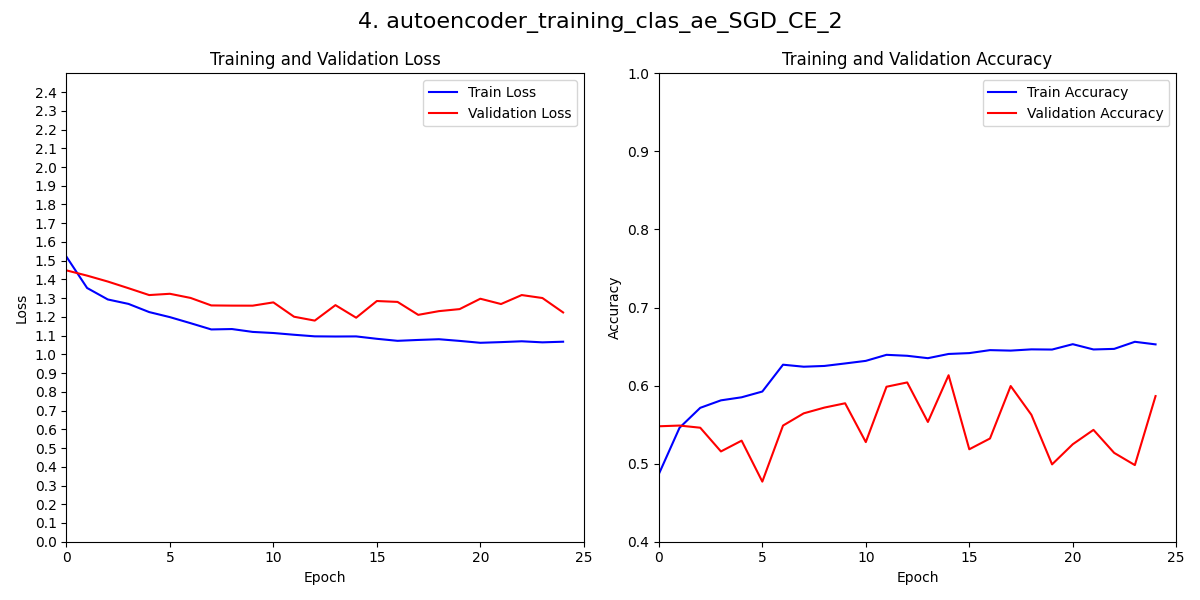
\includegraphics[width=1.\textwidth]{img/aeMMC_sgd_ce.png}
        \caption{Entrenamiento y validación del modelo de clasificación usando un \textit{autoencoder} con pérdida \lstinline|categorical_crossentropy|.}
        \label{fig:sgd_ce}
    \end{minipage}
\end{figure}

En el siguiente modelo, se utiliza como función de coste \lstinline|categorical_crossentropy|. Podemos observar en la figura \ref{fig:sgd_ce} como obtiene una la función de pérdida presenta una dinámica diferente. La pérdida de entrenamiento disminuye de manera constante, alcanzando un valor alrededor del 1.1, mientras que la pérdida de validación también disminuye, aunque de manera menos pronunciada, estabilizándose alrededor de 1.3. La precisión de entrenamiento aumenta de manera constante hasta alcanzar aproximadamente 0.7, mientras que la de validación, aunque con más fluctuaciones, muestra una tendencia positiva alcanzando alrededor de 0.6. Este modelo muestra una mejor capacidad de aprendizaje en comparación con el modelo anterior y tiene un buen balance entre la pérdida de entrenamiento y validación, lo que sugiere que es capaz de generalizar mejor.

La diferencia de rendimiento entre \lstinline|mse| y \lstinline|categorical_crossentropy| en los modelos de clasificación se debe a sus diferentes enfoques hacia la salida esperada. MSE, al penalizar las diferencias cuadrática, puede no ajustarse adecuadamente a problemas de clasificación multiclase que requieren distribuciones de probabilidad sobre las clases. Por otro lado, \lstinline|categorical_crossentropy| está diseñado específicamente para este tipo de problemas, evaluando la distancia entre la distribución predicha y la distribución real de las clases. En el análisis presentado, el modelo que utiliza \lstinline|categorical_crossentropy| mostró una mejor capacidad para aprender y generalizar, reflejado en unos resultados más favorables en comparación con el modelo que emplea \lstinline|mse|.



\subsection{Autoencoder profundo}

No tenemos que limitarnos a una sola capa como codificador o decodificador, en su lugar podríamos usar una pila de capas. El segundo método que vamos a abordar para resolver este problema de clasificación en usando un \textit{autoencoder} con 3 capas densas en el \textit{encoder} y otras tres capas densas en el \textit{decoder}. En la figura \ref{img: daeMMC} podemos ver su arquitectura y el número de neuronas en cada capa. Se ha decidido ese número de neuronas en base a poder tener una red profunda de capas densas sin llegar a perjudicar computacionalmente el problema. Aun así, al aumentar el número de capas y de parámetros con respecto al modelo anterior, el tiempo de entrenamiento de cada época se multiplica por 4. 

\begin{figure}[h]
    \begin{center}
    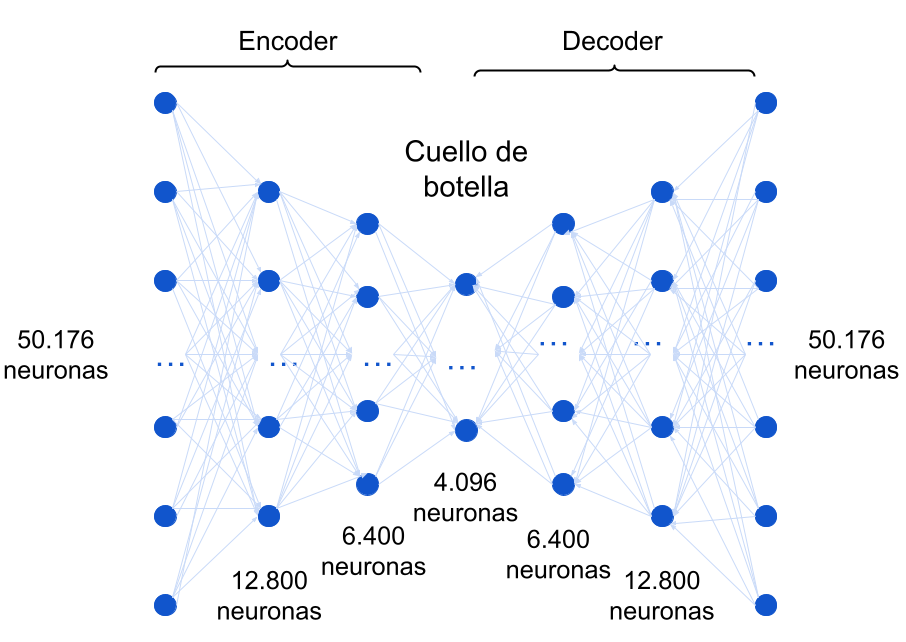
\includegraphics[width=0.4\textwidth]{img/daeMMC.png}
    \end{center}
    \caption{Esquema de la arquitectura usando un \textit{autoencoder} profundo.}
    \label{img: daeMMC}
\end{figure}

Al igual que en el modelo anterior, como vamos a usar capas densas, es necesario que los datos de entrada estén aplanados en un vector de dimensión $50.176$. Este modelo se entrenará durante 25 épocas y con mini-lotes de 8. Se usará el optimizador Adam y función de pérdida \lstinline|mse| como ya se comentó antes. Al acabar el entrenamiento, obtenemos una pérdida en los datos de entrenamiento del 0.04027 y en los datos de validación ($20\%$ del total), un 0.04053. A pesar de que el modelo nos mostraba indicios de que podía seguir mejorando su rendimiento, debido a su alta carga computacional, decidimos parar su entrenamiento en su vuelta 25 ya que sus resultado ya mejoran a los del \textit{autoencoder} con 1 única capa oculta. Con esta nueva representación comprimida de los datos, se vuelve a aplicar la capa de clasificación pero ahora solo con optimizador SGD y función de pérdida \lstinline|categorical_crossentropy|.

\begin{figure}[H]
    \centering
    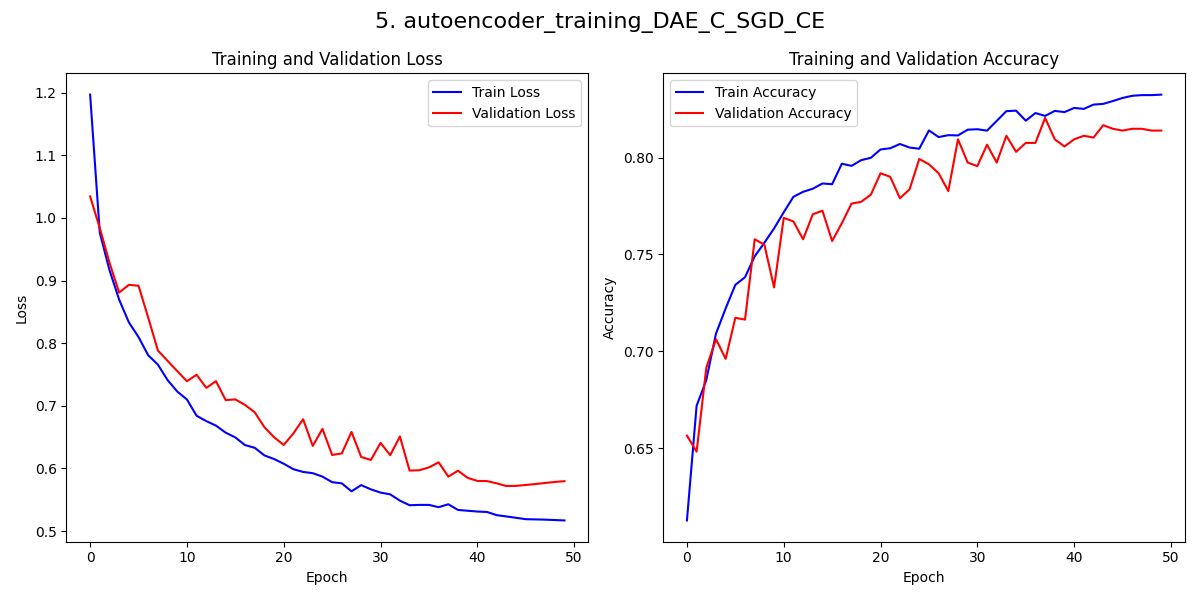
\includegraphics[width=0.5\textwidth]{img/daeMMC_sgd_ce.png}
    \caption{Entrenamiento y validación del modelo de clasificación usando un \textit{autoencoder} profundo}
    \label{fig:dae_sgd_mse}
\end{figure}


A continuación, se crea la misma arquitectura que en el ejemplo anterior para clasificación. Entrenamos el modelo durante 50 épocas con mini-lotes de 8. En la gráfica proporcionada con los resultados obtenidos, se observa el comportamiento de las curvas de pérdida y precisión tanto para el conjunto de entrenamiento como para el de validación. La pérdida de entrenamiento disminuye constantemente desde un valor inicial cercano a 1.2 hasta aproximadamente 0.5, lo que indica un buen ajuste del modelo a los datos de entrenamiento. La pérdida de validación también baja, aunque de manera más moderada, desde cerca de 1.0 hasta alrededor de 0.65 en la época 30. Posteriormente, el \lstinline|val_loss| muestra fluctuaciones y se estabiliza en torno a 0.57 a partir de la época 44, sugiriendo que el modelo ha dejado de mejorar significativamente en términos de generalización. La precisión de entrenamiento incrementa consistentemente de 0.62 a aproximadamente 0.83, mientras que la precisión de validación, aunque inicialmente ascendente, se estabiliza alrededor de 0.82 después de la época 44, reflejando un estancamiento en la mejora del modelo para los datos de validación. Este patrón sugiere que el modelo ha alcanzado su capacidad óptima de generalización, y futuras mejoras en la precisión de entrenamiento no se reflejan en los datos de validación.

Comparado con el modelo anterior, este modelo muestra un mejor rendimiento en todas sus métricas, tanto en la pérdida como en la precisión, lo que sugiere una mejor capacidad de aprendizaje. La arquitectura mejorada de este modelo, con más capas ocultas en el \textit{autoencoder}, permite un aprendizaje más profundo y efectivo, resultando en un ajuste más fino a los datos de entrenamiento y una mejor generalización.



\subsection{Autoencoder convolucional}

Por último, como nuestros datos de entrada los tenemos agrupados en imágenes, se nos ha ocurrido utilizar redes neuronales convolucionales como codificadores y decodificadores. Para ello, se van a utilizar capas convolucionales y capas de \textit{max pooling} como \textit{encoders} y capas convolucionales y de \textit{upsampling} como \textit{decoders}. En la imagen \ref{img: caeMMC} se muestra la arquitectura de este modelo. Se ha seguido la arquitectura propuesta por Kayikcci et al. \citep{kayikcci2020convolutional} en su artículo \textit{Convolutional Autoencoder Model for Reproducing Fingerprint} añadiendo alguna capa extra para llegar al cuello de botella con una dimensión exacta que en la CNN, $7 \times 7$ con 512 mapas de características.

\begin{figure}[h]
    \begin{center}
    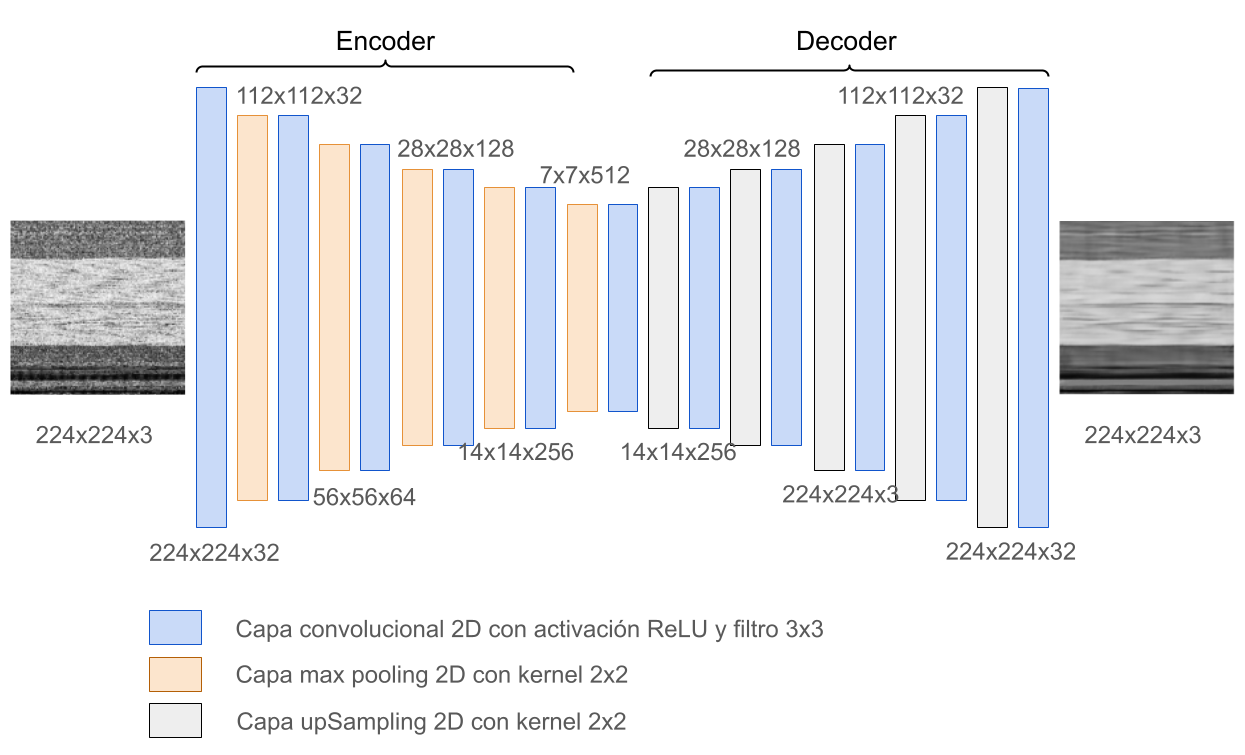
\includegraphics[width=0.7\textwidth]{img/caeMMC.png}
    \end{center}
    \caption{Esquema de la arquitectura usando un \textit{autoencoder} convolucional.}
    \label{img: caeMMC}
\end{figure} 

Este modelo se entrenará durante 100 épocas y con mini-lotes de 8. Se usará el optimizador Adam y función de pérdida \lstinline|mse| como ya se comentó antes. Al acabar el entrenamiento, observamos que la pérdida en la segunda época ya mejora la perdida obtenida en los otros dos modelos anteriores, con un 0.03967 en los datos de entrenamiento y un 0.03885en los datos de validación. Después de las 100 vueltas, obtenemos 0.03528 en los datos de entrenamiento y 0.03498 en los datos de validación. A pesar de que el modelo nos mostraba indicios de que podía seguir mejorando su rendimiento, debido a su alta descenso continuo de la pérdida en los valores de entrenamiento y validación, se decide parar en la vuelta 100 debido a sus excelentes resultados obtenido hasta ese momento. En la imagen \ref{img: reprComprimMMC}, podemos ver como funciona nuestro \textit{autoencoder} convolucional y como la predicción de nuestro modelo se asemeja bastante a la imagen original. 
\begin{figure}[h]
    \begin{center}
    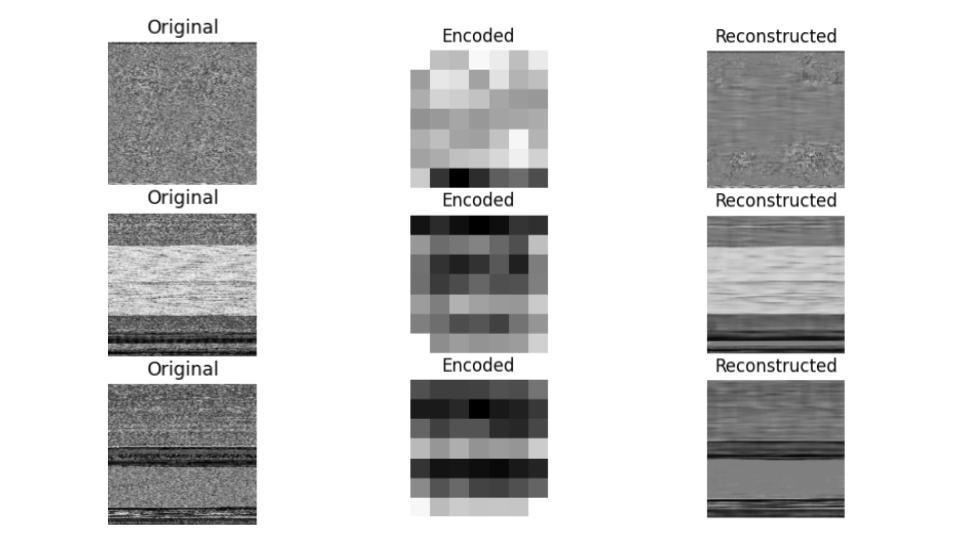
\includegraphics[width=0.52\textwidth]{img/reprComprimMMC.png}
    \end{center}
    \caption{Visualización de la imagen original, versión comprimida y versión decodificada usando el \textit{autoencoder} convolucional.}
    \label{img: reprComprimMMC}
\end{figure}

\bigskip

Con esta nueva representación comprimida de los datos, se vuelve a aplicar la capa de clasificación con optimizador SGD y función de pérdida \lstinline|categorical_crossentropy| que vimos en la sección \ref{3.cnn} de la CNN.

\begin{figure}[H]
    \centering
    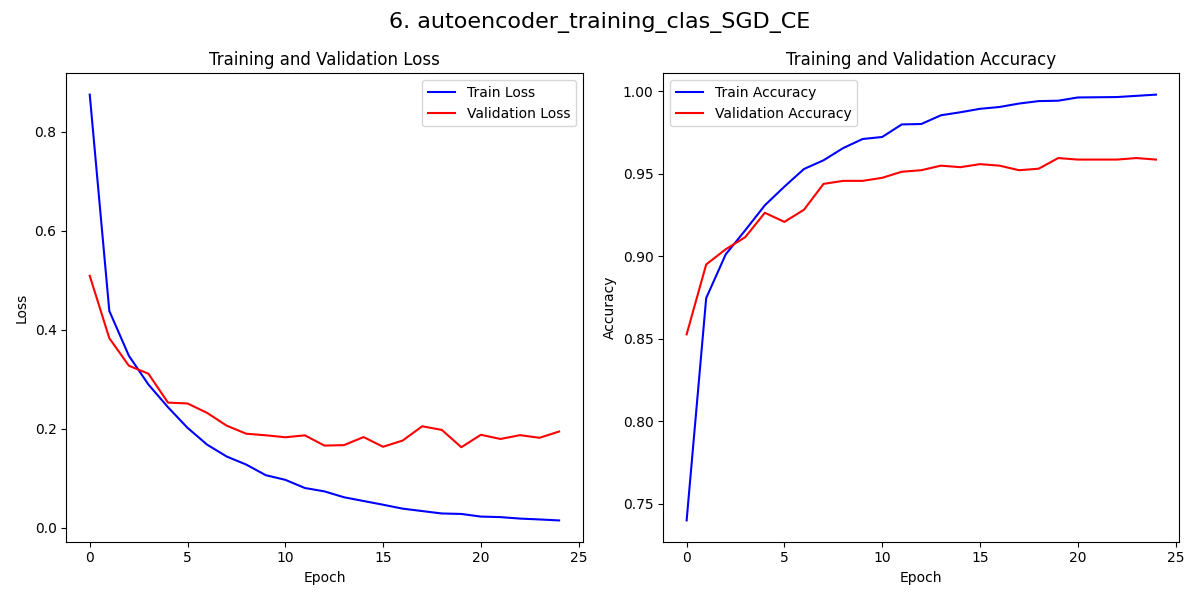
\includegraphics[width=0.6\textwidth]{img/caeMMC_sgd_ce.png}
    \caption{Entrenamiento y validación del modelo de clasificación usando un \textit{autoencoder} convolucional.}
    \label{fig:resultados_cae}
\end{figure}

En la Figura \ref{fig:resultados_cae} se observa el comportamiento de las curvas de pérdida y precisión tanto para el conjunto de entrenamiento como para el de validación a lo largo de 25 épocas. La pérdida de entrenamiento disminuye de manera constante desde un valor inicial cercano a 0.9 hasta aproximadamente 0.015, indicando un buen ajuste del modelo a los datos de entrenamiento. La pérdida de validación también decrece, aunque de manera más moderada, desde cerca de 0.5 hasta estabilizarse alrededor de 0.2 a partir de la época 12, sugiriendo que el modelo ha dejado de mejorar significativamente en términos de generalización. La precisión de entrenamiento incrementa consistentemente de 0.85 a aproximadamente 1, mientras que la precisión de validación, aunque inicialmente asciende, se estabiliza alrededor de 0.95 después de la época 12, reflejando un estancamiento en la mejora del modelo para los datos de validación. Sin embargo, dado que el modelo utiliza \textit{EarlyStopping} con restauración de los pesos del mejor modelo, se ha guardado el estado del modelo en el punto donde mejor generaliza, mitigando así el impacto del \textit{overfitting}.







 
\begin{comment}
\subsection{CAE}
parametros de optimizador y loss: \citep{guo2017deep}
En AE se decide escoger MSE porque queremos medir regresión, no clasificación
\subsection{DAE}
Para el resto de modelos hemos usado las mismas funciones para poder comparar parámetros
\subsection{AE}
Convolutional autoencoder modelo \citep{xing2022malware}
\end{comment}


\newpage

\section{Resultados}

En esta sección, se presentan y analizan los resultados obtenidos a partir de los diversos experimentos realizados. Se han explorado diferentes enfoques, incluyendo una \acrshort{cnn} con técnicas de regularización como \textit{dropout} y \lstinline|EarlyStopping|, y tres tipos de \textit{autoencoders}: simple, profundo y convolucional. De cada uno de estos enfoques se escogió el que tenía mejor rendimiento para ahora comparar ambos y quedarse con el modelo final para este problema de clasificación. A continuación, se detallan los resultados y conclusiones obtenidos de estos experimentos.


\subsubsection*{CNN con dropout y EarlyStopping}
Tras definir la arquitectura de la CNN siguiendo el artículo \citep{kalash2018malware} y realizar múltiples experimentos, encontramos que el modelo inicial, aunque alcanzaba un \textit{accuracy} del 0.959 en el conjunto de validación, presentaba signos de sobreajuste. Para mejorar la generalización, se añadieron capas de \textit{dropout} y se implementaron técnicas como \lstinline|EarlyStopping|. Los resultados mostraron que una tasa de \textit{dropout} del 0.5, combinada con la estrategia de detener el entrenamiento temprano, proporcionó el mejor balance entre precisión y capacidad de generalización, logrando un \textit{accuracy} del 0.965 y un \textit{loss} del 0.17 en validación. Estos ajustes permitieron mejorar significativamente el rendimiento del modelo. Para evaluar el rendimiento de este modelo en el problema de Microsoft Malware Classification, se ha generado una matriz de confusión con los datos de prueba que ya habíamos reservado para este análisis (15\% del total). A continuación, se procederá a calcular y analizar las métricas de precisión, TPR (sensibilidad), FPR, F1 Score, y proponer mejoras basadas en estos resultados.

\begin{figure}[H]
    \centering
    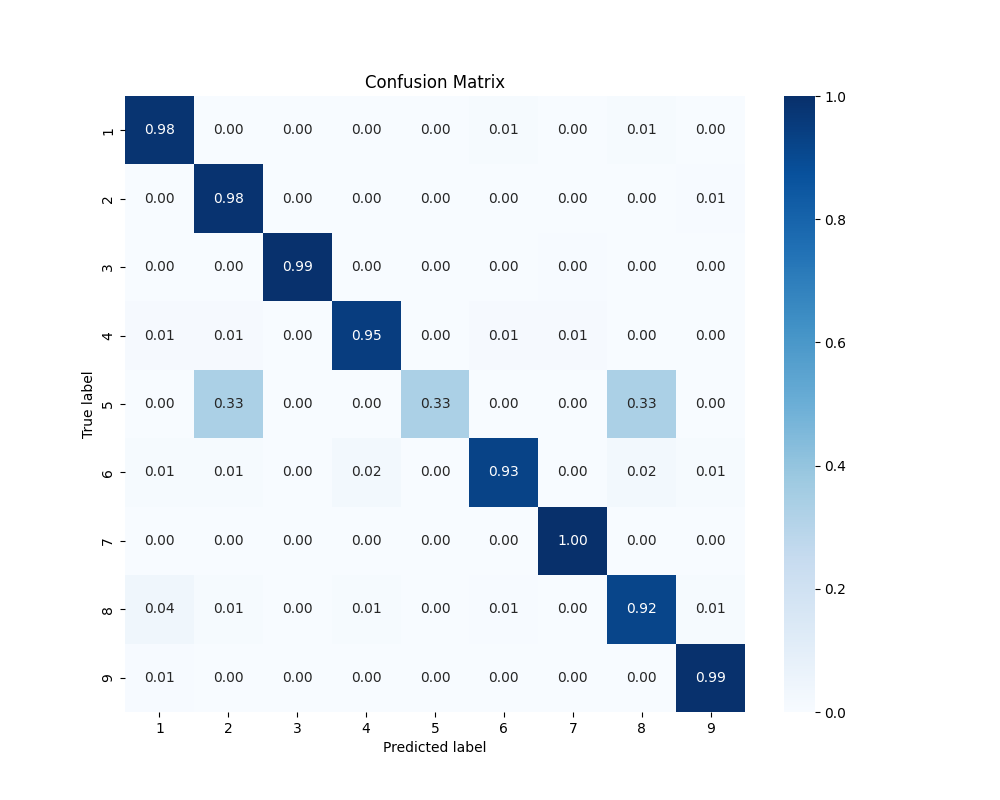
\includegraphics[width=0.6\textwidth]{img/confusionMatrixCNNNormal1.png}
    \caption{Matriz de confusión del modelo utilizando una \acrshort{cnn}.}
    \label{fig: cnnConfusionMatrix}
\end{figure}

En la figura \ref{fig: cnnConfusionMatrix} se observa que la mayoría de las predicciones están bien clasificadas, ya que la diagonal principal de la matriz tiene los valores más altos (en azul oscuro), lo que indica un porcentaje mayor a 0.9. Sin embargo, hay algunas clases que no siguen este patrón, como la clase con etiqueta 5, que corresponde al tipo de malware Simbda. Esta clase obtiene un 33\% de éxito, lo que contrasta con el resultado global de éxito (96.5\%). Estos resultados sugieren que el modelo no ha generalizado adecuadamente para la clase 5, probablemente debido al bajo número de muestras en el dataset, ya que solo representa el 0.4\% del total.

\begin{table}[H]
    \centering
    \begin{tabular}{|c|c|c|c|c|}
        \hline
        \textbf{Clase} & \textbf{Precisión} & \textbf{TPR (Sensibilidad)} & \textbf{FPR} & \textbf{F1 Score} \\
        \hline
        1 & 0.98 & 0.98 & 0.01 & 0.98 \\
        2 & 0.98 & 0.98 & 0.00 & 0.98 \\
        3 & 0.99 & 0.99 & 0.00 & 0.99 \\
        4 & 0.95 & 0.95 & 0.00 & 0.95 \\
        5 & 0.33 & 0.33 & 0.67 & 0.33 \\
        6 & 0.93 & 0.93 & 0.02 & 0.93 \\
        7 & 1.00 & 1.00 & 0.00 & 1.00 \\
        8 & 0.92 & 0.92 & 0.01 & 0.92 \\
        9 & 0.99 & 0.99 & 0.00 & 0.99 \\
        \hline
    \end{tabular}
    \caption{Métricas de evaluación por clase para el modelo \acrshort{cnn}.}
    \label{tab: cnnMetrics}
\end{table}

Las métricas de la tabla \ref{tab: cnnMetrics} muestran un alto rendimiento para la mayoría de las clases, con F1 Scores que oscilan entre 0.92 y 1.00 para las clases 1, 2, 3, 4, 6, 7, 8 y 9. La clase 5, sin embargo, presenta un rendimiento significativamente inferior, con una precisión de 0.33, una sensibilidad de 0.33 y un F1 Score de 0.33, lo que indica dificultades en identificar correctamente los ejemplos de esta clase.

Para mejorar el rendimiento del modelo en la clase 5, se podría utilizar la técnica de pesos de clase \citep{amoros2021desbalanceo}. Esta técnica consiste en asignar un peso específico a cada clase dentro de la red neuronal, permitiendo que la red preste más atención a aquellas clases con un peso mayor. Para determinar estos pesos, deben calcularse usando la siguiente fórmula:

\[
W_j = \sqrt{\frac{s}{c \cdot S_j}}
\]

Donde $W_j$ representa el peso de la clase $j$, $s$ es el número total de muestras, $c$ es el número total de clases y $S_j$ es el número de muestras de la clase $j$. Estos pesos se emplean durante el cálculo de la función de pérdida. Una vez que se ha calculado la pérdida para cada clase, esta se multiplica por el peso correspondiente de la clase. Este procedimiento permite ``balancear'' la importancia relativa de cada clase durante el entrenamiento de la red.

\subsubsection*{Autoencoder convolucional}
En la segunda parte del cápitulo \ref{Capitulo_2}, hemos explorado tres tipos de \textit{autoencoders}: un \textit{autoencoder} simple, un \textit{autoencoder} profundo, y un \textit{autoencoder} convolucional, cada uno evaluado en términos de pérdida y precisión tanto en entrenamiento como en validación. Los resultados muestran que el \textit{autoencoder} convolucional destaca por su capacidad superior de compresión y generalización, alcanzando una precisión de validación del 95.8\% y una pérdida de validación de 0.192, superando significativamente a los \textit{autoencoders} simples y profundos. Mientras que el \textit{autoencoder} simple con una sola capa oculta presentó limitaciones en su capacidad de generalización, el \textit{autoencoder} profundo mostró mejoras notables, aunque a costa de una mayor complejidad computacional. Por su parte, el \textit{autoencoder} convolucional, al aprovechar la estructura espacial de los datos de entrada, logró una mayor precisión y una menor pérdida, estableciendo un gran equilibrio entre la complejidad del modelo y la capacidad de generalización, convirtiéndose así en la opción más precisa para esta tarea de clasificación.


Para evaluar el rendimiento del \textit{autoencoder} convolucional en el problema de Microsoft Malware Clasification, se ha generado una matriz de confusión (Figura \ref{fig: caeConfusionMatrix}) con los datos de prueba. 


\begin{figure}[H]
    \centering
    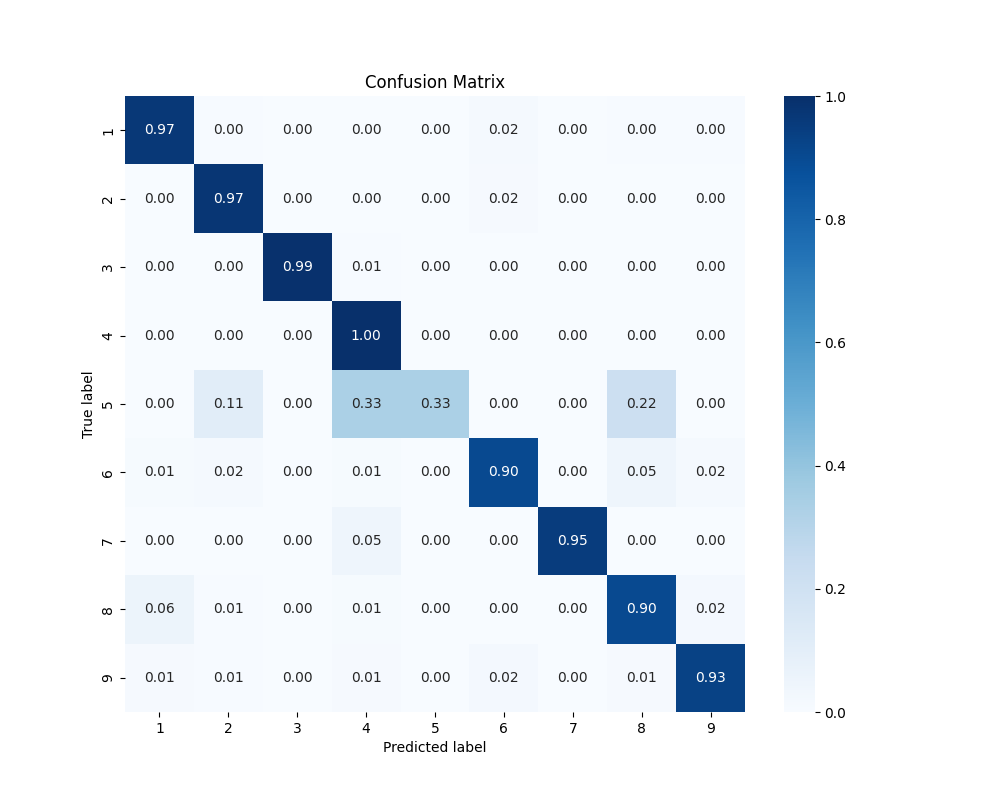
\includegraphics[width=0.6\textwidth]{img/confusionMatrixCAENorm1.png}
    \caption{Matriz de confusión del modelo utilizando un \textit{autoencoder} convolucional.}
    \label{fig: caeConfusionMatrix}
\end{figure}


En ella se puede observar como la mayoría de las predicciones están bien clasificadas al igual que para la \acrshort{cnn}, pero la clase con etiqueta 5 obtiene un 33\% de éxito también.
 
Además en la tabla \ref{tab:metrics}, se puede observar una alta precisión y sensibilidad en la mayoría de las clases, con F1-scores que oscilan entre 0.89 y 0.98, lo que indica un gran equilibrio entre la precisión y la sensibilidad. La clase 3 sobresale con un F1-score de 0.98, reflejando una excelente precisión (0.97) y sensibilidad (0.99). Sin embargo, la clase 5 presenta un rendimiento significativamente inferior, con una precisión de 0.49, una sensibilidad de 0.33 y un F1-score de 0.39, señalando que el modelo tiene dificultades en identificar los ejemplos de esta clase. Este problema, al igual que con la \acrshort{cnn}, podría resolverse usando pesos de clase. 


\begin{table}[H]
\centering
\begin{tabular}{|c|c|c|c|c|}
\hline
Clase & Precisión & TPR (Sensibilidad) & FPR & F1 Score \\ \hline
1 & 0.94 & 0.97 & 0.06 & 0.96 \\ \hline
2 & 0.92 & 0.97 & 0.07 & 0.94 \\ \hline
3 & 0.97 & 0.99 & 0.03 & 0.98 \\ \hline
4 & 0.91 & 1.00 & 0.09 & 0.95 \\ \hline
5 & 0.49 & 0.33 & 0.06 & 0.39 \\ \hline
6 & 0.94 & 0.90 & 0.03 & 0.92 \\ \hline
7 & 0.95 & 0.95 & 0.05 & 0.95 \\ \hline
8 & 0.88 & 0.90 & 0.12 & 0.89 \\ \hline
9 & 0.94 & 0.93 & 0.06 & 0.94 \\ \hline
\end{tabular}
\caption{Métricas de rendimiento por clase en el \textit{autoencoder} convolucional.}
\label{tab:metrics}
\end{table}

En conclusión, a pesar de que tanto la \acrshort{cnn} como el \textit{autoencoder} convolucional presentan buenos resultados en general, la \acrshort{cnn} demostró un mejor rendimiento en términos de \textit{accuracy} y \textit{loss} en el conjunto de validación, logrando un equilibrio óptimo entre precisión y capacidad de generalización. Este mejor rendimiento puede atribuirse a la estructura de la \acrshort{cnn}, que es especialmente adecuada para capturar características espaciales complejas en los datos de entrada. Además, las técnicas implementadas, como el \textit{dropout} y el \textit{early stopping}, permitieron optimizar el modelo y prevenir el sobreajuste, haciendo de la \acrshort{cnn} la opción más efectiva para el problema de \textit{Malware Microsoft Clasiffication Challenge (BIG 2015)}.





\begin{comment}

\begin{figure}[h]
    \begin{center}
    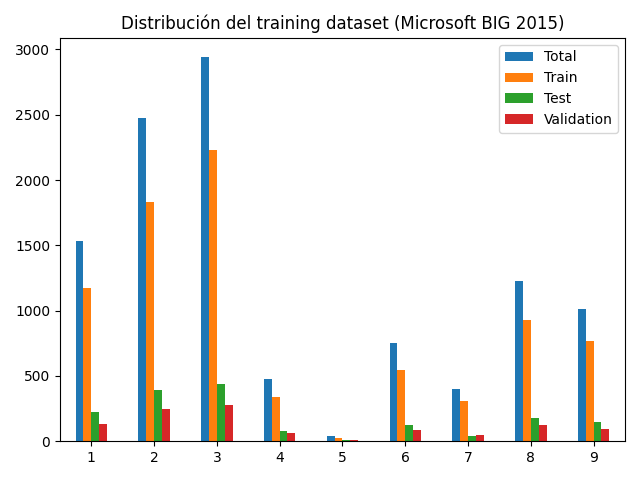
\includegraphics[width=0.6\textwidth]{img/barras4MMC.png}
    \end{center}
    \caption{Distribución de las clases en cada grupo.}
    \label{img: train_test_valMMC}
\end{figure}

\section{Resumen del Conjunto de Datos}

El conjunto de datos utilizado en este estudio proviene del Desafío de Clasificación de Malware de Microsoft (BIG 2015), accesible a través de Kaggle. Este conjunto de datos consta de programas de malware pertenecientes a 9 categorías diferentes. Se proporcionan conjuntos de datos de entrenamiento y prueba, pero solo se utilizan los datos de entrenamiento debido a la falta de etiquetas para el conjunto de prueba para su entrega. Además

El conjunto de entrenamiento contiene 10,868 muestras de malware, cada una con un identificador único, un valor hash de 20 caracteres y una etiqueta de clase que representa una de las 9 familias de malware. Cada archivo de malware tiene una representación hexadecimal de su contenido binario, junto con un archivo 'bytes' que contiene esta información. No se excluye ninguna categoría de malware en este estudio.

La distribución de los datos se realiza con un 72\% para entrenamiento, un 8\% para validación y un 20\% para pruebas. Se realizan varias divisiones y análisis de los conjuntos de datos para ajustar y evaluar diferentes modelos y enfoques de aprendizaje profundo para la clasificación de malware.

Este conjunto de datos, con su amplia gama de muestras etiquetadas y la diversidad de familias de malware representadas, proporciona una base sólida para la investigación y desarrollo de métodos efectivos de detección y clasificación de amenazas informáticas.













\item Worm (Gusano)- Los gusanos informáticos son un tipo de malware que puede propagarse a través de redes sin la intervención de un programa huésped o de un humano. Son caballos de Troya maliciosos que pueden replicarse y propagarse de una computadora a otra. Los gusanos infectan a sus anfitriones mediante el engaño y la astucia, pudiendo causar graves daños a las computadoras comprometidas al consumir ancho de banda, sobrecargar sistemas, eliminar o modificar archivos e instalar virus adicionales. Además, las vulnerabilidades en el software, los archivos adjuntos de correo electrónico y las conexiones de red pueden facilitar su propagación. 

\item Adware (programa publicitario) - El adware es una variedad de malware que muestra anuncios no deseados a los usuarios, típicamente como ventanas emergentes o banners. A menudo se distribuye como parte de descargas de software gratuitas, pero también se puede obtener a través de un ciberataque o una vulnerabilidad. El adware tiene como objetivo generar ingresos para sus desarrolladores mostrando anuncios a los consumidores. Sin embargo, puede causar un daño significativo a una computadora infectada al degradar su rendimiento, reducir su disponibilidad y violar la privacidad del usuario al recopilar información sobre sus actividades de navegación.

\item Backdoor (Puerta trasera) - Un backdoor permite que una entidad no autorizada tome el control completo del sistema de una víctima sin su consentimiento. Un troyano de puerta trasera siempre se presenta como una herramienta de software legítima esencialmente requerida por el usuario. Otras opciones pueden ser visitar un sitio web malicioso o hacer clic en un enlace no deseado. Al ejecutarse, se añade a sí mismo en la rutina de inicio del sistema y busca una conexión a Internet. Una vez que el sistema está en línea, se conecta con su autor, quien luego toma el control del sistema para realizar diferentes tareas, como descargar/cargar archivos, registrar pulsaciones de teclas, enviar correos electrónicos no deseados o robar contraseñas, entre otras cosas.

\item Trojan (Troyano)- Los troyanos son programas maliciosos que se disfrazan como programas o archivos legítimos y pueden tomar el control de una computadora para ejecutar operaciones maliciosas como robar datos, dañar el sistema o abrir puertas traseras para otros virus. El término "Troyano" proviene de la leyenda griega del caballo de Troya, una táctica engañosa utilizada para conquistar Troya. En el ámbito digital, los troyanos son parásitos digitales hostiles capaces de leer contraseñas, grabar pulsaciones de teclas y propagar otros virus. Se utilizan técnicas de ingeniería social, como correos electrónicos de phishing o descargas maliciosas, para propagarlos. A diferencia de los virus informáticos y los gusanos, los troyanos no pueden replicarse y deben ser instalados o ejecutados por los usuarios.

\item Trojan downloader (Descargador troyano) - Es un programa malicioso que se descarga e instala en una computadora infectada. Puede abrir conexiones de red ilícitas, mutarse a sí mismo, deshabilitar herramientas de seguridad y transferir información personal del usuario sin permiso. Además, su función principal es la de descargar e instalar otro malware dañino en el sistema infectado.

\item Obfuscated malaware (Malware obfuscado) - La obfuscación es una técnica utilizada para hacer que el código de un programa sea más difícil de entender o de analizar. Esto implica modificar el código del programa malicioso de manera que sea más complicado para los investigadores de seguridad o los programas antivirus detectarlo y comprender cómo funciona. Su objetivo principal es eludir la detección y análisis por parte de los programas antivirus y otros sistemas de seguridad.













\item Ramnit es un malware de tipo gusano detectado en el 2011 y que afecta sistemas operativos Windows. , pueden ser utilizadas para múltiples objetivos maliciosos. Ramnit es una avanzada herramienta para criminales con funcionalidades de rootkit, no detección por antivirus, inyección Web y uso de comunicaciones cifradas con el centro de Comando y Control. Ramnit es un malware que ha sido utilizado para realizar actividades criminales, entre las que se pueden destacar. Monitorización de la navegación web del sistema infectado y detectar la visita de sitios de banca online. Manipulación de webs de banca online con el objetivo de parecer legitimar. Robo de cookies de sesión de los navegadores web para poder suplantar a la víctima en sitios seguros. Escaneo los discos duros de la computadora y robo archivos en base a palabras clave (como contraseñas). Acceso de forma remota a los ordenadores afectados. Recopilación de las credenciales de acceso de clientes de FTP.
¿Cómo me infecta? Se cree que su propagación es través de enlaces de confianza enviados a través de correos electrónicos de phishing o mediante redes sociales, que están principalmente orientados principalmente al robo de dinero de cuentas bancarias de victimas con sistemas operativos Windows. También se ha detectado el uso servidores FTP públicos para la distribución del malware.


\item Lollipop (L) is an adware that produces profits for the developer by automatically showing advertisements on the user
computer.
\item 1 Swizzor Swizzor is a type of malware flies that under the radar to deliver unsolicited advertisements, modifying browser setting without
user permission.
2 Vundo Vundo is either a Trojan horse or a computer worm that is known to cause Pop-up advertising for rogue antispyware programs.
3 Spybot Spybot is a type of worm that usually arrives on a computer through peer-to-peer file sharing, specifically through the Kazaa file
sharing network. Its many variants sometimes have other ways of spreading.
4 Ransom Ransom is a type of malware that can be covertly installed on a computer without knowledge or intention of the user that
restricts access to the infected computer system in some way, and demands that the user pay a ransom to the malware
operators to remove the restriction.
5 Ramnit Ramnit is a type of virus that infects Windows executable files and HTML files. It can also give a malicious hacker access to
your computer. It spreads through infected removable drives, such as USB flash drives.
6 Lollipop Lollipop is a type of adware program that shows advertisements as you browse the web. It can also redirect your search engine
results, monitor what you do on your computer, download applications, and send information about your computer to a hacker.
7 Kelihos Kelihos is a type of trojan that can give a malicious hacker access and control of your computer. The family spreads by sending
spam emails that have links to other malware.
8 Delf Delf is a type of trojan that reports and intercepts Internet traffic and may also download unwanted applications onto your
computer.
9 Banker Banker is a type of data-stealing trojans that can capture your online banking details, such as your log 

\citep{tang2019dynamic}

\item Simda es un malware de tipo troyano que infecta ordenadores con sistema operativo Windows. Los ordenadores infectados con este malware pasan a ser parte de una botnet, con lo que pueden ser utilizados para cometer acciones criminales o maliciosas.

¿Qué hace?	
Esta familia de malware incluye funcionalidades de backdoor, robo de contraseñas, robo de credenciales bancarias y es capaz de descargar otro tipo de malware.

Sistemas afectados	
Principalmente sistemas Windows:

Windows XP
Windows Vista
Windows 7
Windows 8
¿Cómo me infecta?	
El contagio de esta amenaza es mediante la distribución de archivos previamente infectados o a través de redes compartidas.

\item Obfuscation malware, also known as obfuscation techniques or code obfuscation, is a strategy employed by cybercriminals to hide the true intent and functionality of their malicious code. Essentially, it’s a way of making malware more difficult to detect and analyze by security software and researchers.

Compression, encryption, and encoding are some of the most common obfuscation methods used by threat actors. Multiple methods are often used in tandem to evade a wider variety of cyber security tools at the initial point of intrusion.

\item Gatak is a backdoor trojan that first appeared in 2012. Another name for this threat is Stegoloader, and its main distinctive feature is its ability to communicate with its C&C servers via steganography.

El grupo detrás de Trojan Gatak (Trojan.Gatak) continúa siendo una amenaza para las compañías, especialmente para el sector salud, fuertemente impactado por los ataques. Gatak es conocido por infectar a sus víctimas por medio de sitios web que prometen claves de licencias de producto para software pirata. Si bien el grupo se enfocó inicialmente en blancos en los Estados Unidos, a lo largo de los últimos dos años se ha diversificado y los ataques se llevan a cabo ahora contra compañías en varios países.

La mayor parte de las infecciones de Gatak (62%) ocurre en computadoras corporativas. El análisis de recientes ataques corporativos indica que el sector de la salud es, sin lugar a dudas, el más impactado por Gatak. De las 20 principales compañías más afectadas (compañías con más computadoras infectadas), 40% eran en el sector de la salud. En el pasado, el sector de seguros también quedó fuertemente en la mira del grupo.

Sitio web de generación de claves para licencias usado para atraer a las víctimas inocentesLas víctimas de Gatak son infectadas usando sitios web que ofrecen generar claves para licencias de productos o "keygens" de software pirata. El malware es empaquetado con la clave del producto y, si la víctima es inducida a bajar y abrir uno de esos archivos, el malware se instala clandestinamente en su computadora.

Los responsables del ataque parecen enfocarse en ofrecer claves de producto para softwares que son más probables que se utilicen en entornos profesionales. Los sitios web usados ​​en los ataques son controlados por los grupos de ataque y no tienen relación con los desarrolladores del software. En ningún momento se comprometen las versiones legítimas del software. Entre las marcas de softwares usadas ​​como anzuelos se han identificado:
SketchList3D (software de diseño para carpintería)
Native Instruments Drumlab (software de ingeniería de audio)
BobCAD-CAM (software de manufactura/metalúrgica)
BarTender Enterprise Automation (software de creación de etiquetas y código de barras)
HDClone (utilitario de clonaje de disco rígido)
Siemans SIMATIC STEP 7 (software de automación industrial)
CadSoft Eagle Professional (software de diseño de placa de circuito impreso)
PremiumSoft Navicat Premium (software de administración de base de datos)
Originlab Originpro (software gráfico para análisis de datos)
Manctl Skanect (software de digitalización 3D)
Symantec System Recovery (software de backup y recuperación de datos; ahora parte de Veritas)
Las claves de producto bajadas a partir de estos sitios no funcionan y simplemente generan una secuencia pseudoaleatoria de caracteres. Eso significa que todo lo que la víctima recibe con la descarga es un archivo inútil y una posible infección de Gatak.
Herramientas de Malware
Trojan Gatak (también conocido por Stegoloader) ha sido utilizado en ataques por lo menos desde 2011. Existen dos componentes principales de malware. Un módulo de implementación leve (Trojan.Gatak.B) puede realizar una identificación detallada del sistema en las computadoras infectadas e instalar selectivamente cargas adicionales. El módulo principal (Trojan.Gatak) es un verdadero Troyano de backdoor, que mantiene una presencia persistente en una computadora infectada y roba su información.

Una característica notable de Gatak es el uso de esteganografía, una técnica que esconde datos dentro de archivos de imagen. Cuando Gatak se instala en una computadora, intenta bajar un archivo de imagen PNG de una serie de direcciones URL codificadas en el malware. La imagen se parece a una fotografía común, sin embargo, contiene un mensaje cifrado dentro de sus datos de pixel. Trojan Gatak es capaz de decodificar este mensaje, que contiene comandos y archivos para su ejecución.
En casi el 62% de los incidentes, el movimiento lateral en la red de la víctima se produce dentro de las dos horas tras la infección. En los casos restantes, el movimiento lateral se inició en algún momento después de dos horas. La variación indica que el movimiento lateral no es automático, sino que se ejecuta manualmente por los grupos de ataque. No se sabe con precisión si los grupos de ataque poseen los recursos para explorar todas las infecciones inmediatamente o si ellos priorizan algunas infecciones sobre otras.

Poco se sabe acerca de cómo los grupos de ataque se mueven en la red de una compañía. La explicación más probable es que ellos exploran contraseñas débiles y una seguridad pobre en archivos compartidos y en las unidades de red. No existe evidencia de ataques de día cero o que se empleen herramientas sofisticadas de hacking.

En algunos casos, los grupos de ataque infectaron computadoras con otros tipos de malware, incluso varias variantes de ransomware y el Troyano financiero Shylock (Trojan.Shylock). En el caso de Shylock, estas parecen ser versiones más antiguas de la amenaza y pueden incluso ser infecciones de "bandera falsa". Pueden utilizarse ​por el grupo cuando creen que su ataque fue descubierto, a fin de engañar a los investigadores.
¿Por qué el área de la salud?
Poco se sabe acerca del grupo responsable de Gatak, si bien la naturaleza corporativa de sus blancos, en conjunto con la ausencia de vulnerabilidades de día cero o módulos de malware avanzados, sugieren que pueden ser cibercriminales en su esencia, aunque también existen recursos dentro del malware para operaciones más tradicionales de espionaje.

No está claro como Gatak está obteniendo lucro con sus ataques. Una posibilidad es el robo de datos, con los grupos de ataque vendiendo información de identificación personal y otros datos robados en el cibermercado clandestino. Esto podría explicar el foco determinado de los grupos de ataque en el sector de la salud, pues los registros con información de salud normalmente se venden a mejores precios comparados con otra información personal.

Sin embargo, los medios de distribución de Gatak, a través de sitios de generación de claves de licencia, indican que los grupos de ataque pueden ser más oportunistas. Al utilizar un abordaje watering-hole, los grupos de ataque desempeñan un papel en gran parte pasivo, con relativamente poco control sobre quien es infectado. Si este es el caso, el sector de la salud puede simplemente ser el más susceptible a este tipo de ataque.

Las compañías de salud muchas veces pueden estar bajo presión, con pocos recursos, y muchas usan sistemas de software legados cuyas actualizaciones son muy caras. Por consiguiente, los profesionales podrían ser más propensos a tomar atajos e instalar software pirata. Si bien parece que las compañías de otros sectores se infectan con menos frecuencia, los grupos de ataque no parecen ignorar o remover esas infecciones cuando se producen.





















un conjunto de datos de malware sin precedentes y promoviendo el desarrollo de técnicas efectivas de código abierto para agrupar variantes de archivos de malware en sus respectivas familias.

Est Fue un challenge que promocionó Microsoft para que la comunidad científica propuesiera una solución para este problema.Es un dataset que fue creado para un Challenge proporcionado por Microsoft para 
Dataset Description
Warning: this dataset is almost half a terabyte uncompressed! We have compressed the data using 7zip to achieve the smallest file size possible. Note that the rules do not allow sharing of the data outside of Kaggle, including bit torrent (why not?).

You are provided with a set of known malware files representing a mix of 9 different families. Each malware file has an Id, a 20 character hash value uniquely identifying the file, and a Class, an integer representing one of 9 family names to which the malware may belong:

Ramnit
Lollipop
Kelihos_ver3
Vundo
Simda
Tracur
Kelihos_ver1
Obfuscator.ACY
Gatak
For each file, the raw data contains the hexadecimal representation of the file's binary content, without the PE header (to ensure sterility).  You are also provided a metadata manifest, which is a log containing various metadata information extracted from the binary, such as function calls, strings, etc. This was generated using the IDA disassembler tool. Your task is to develop the best mechanism for classifying files in the test set into their respective family affiliations.

The dataset contains the following files:

train.7z - the raw data for the training set (MD5 hash = 4fedb0899fc2210a6c843889a70952ed)
trainLabels.csv - the class labels associated with the training set
test.7z - the raw data for the test set (MD5 hash = 84b6fbfb9df3c461ed2cbbfa371ffb43)
sampleSubmission.csv - a file showing the valid submission format
dataSample.csv - a sample of the dataset to preview before downloading

dropout25
Model: "sequential_2"
_________________________________________________________________
 Layer (type)                Output Shape              Param #   
=================================================================
 conv2d_26 (Conv2D)          (None, 224, 224, 64)      1792      
                                                                 
 conv2d_27 (Conv2D)          (None, 224, 224, 64)      36928     
                                                                 
 max_pooling2d_10 (MaxPooli  (None, 112, 112, 64)      0         
 ng2D)                                                           
                                                                 
 conv2d_28 (Conv2D)          (None, 112, 112, 128)     73856     
                                                                 
 conv2d_29 (Conv2D)          (None, 112, 112, 128)     147584    
                                                                 
 max_pooling2d_11 (MaxPooli  (None, 56, 56, 128)       0         
 ng2D)                                                           
                                                                 
 conv2d_30 (Conv2D)          (None, 56, 56, 256)       295168    
                                                                 
 conv2d_31 (Conv2D)          (None, 56, 56, 256)       590080    
                                                                 
 conv2d_32 (Conv2D)          (None, 56, 56, 256)       590080    
                                                                 
 max_pooling2d_12 (MaxPooli  (None, 28, 28, 256)       0         
 ng2D)                                                           
                                                                 
 conv2d_33 (Conv2D)          (None, 28, 28, 512)       1180160   
                                                                 
 conv2d_34 (Conv2D)          (None, 28, 28, 512)       2359808   
                                                                 
 conv2d_35 (Conv2D)          (None, 28, 28, 512)       2359808   
                                                                 
 max_pooling2d_13 (MaxPooli  (None, 14, 14, 512)       0         
 ng2D)                                                           
                                                                 
 conv2d_36 (Conv2D)          (None, 14, 14, 512)       2359808   
                                                                 
 conv2d_37 (Conv2D)          (None, 14, 14, 512)       2359808   
                                                                 
 conv2d_38 (Conv2D)          (None, 14, 14, 512)       2359808   
                                                                 
 max_pooling2d_14 (MaxPooli  (None, 7, 7, 512)         0         
 ng2D)                                                           
                                                                 
 flatten_2 (Flatten)         (None, 25088)             0         
                                                                 
 dense_6 (Dense)             (None, 4096)              102764544 
                                                                 
 dropout_2 (Dropout)         (None, 4096)              0         
                                                                 
 dense_7 (Dense)             (None, 4096)              16781312  
                                                                 
 dropout_3 (Dropout)         (None, 4096)              0         
                                                                 
 dense_8 (Dense)             (None, 9)                 36873     
                                                                 
=================================================================
Total params: 134297417 (512.30 MB)
Trainable params: 134297417 (512.30 MB)
Non-trainable params: 0 (0.00 Byte)
_________________________________________________________________
\end{comment}




